\documentclass[openany,11pt,papersize,dvipdfm,draft]{jsbook}
\usepackage[final]{funpro}
\usepackage{graphicx}
\usepackage{float}

\def\hissu{\bgroup\color{red}}
\def\endhissu{\egroup}

\thisYear{2023}

\jProjectName{使ってもらって学ぶフィールド指向システムデザイン 2023}
\eProjectName{Field Oriented System Design Learning by Users' Feedback 2023}
\ProjectNumber{3-A}
\jGroupName{グループ~A}
\eGroupName{Group~A}

\ProjectLeader{佐々木虎太郎}{Kotaro~Sasaki}
\GroupLeader  {及川寛太}{Kanta~Oikawa}
\SumOfMembers{4}
\GroupMember {1}{及川寛太}{Kanta~Oikawa}
\GroupMember {2}{下村蒔里萌}{Marimo~Shimomura}
\GroupMember {3}{大津武琉}{Takeru~Otsu}
\GroupMember {4}{稲田敬介}{Keisuke~Inada}

\jadvisor{伊藤恵,南部美砂子,奥野拓,元木環,石尾隆}
\eadvisor{Kei~Ito,Misako~Nambu,Taku~Okuno,Tamaki~Motoki,Takashi~Ishio}

\jdate{2024年1月17日}
\edate{January~17, 2024}

\begin{document}
\maketitle

\frontmatter

\begin{jabstract}
 本プロジェクトは,フィールド調査をもとにした活動で発見した問題を,ITを用いて解決する.
これは,ユーザの仕事や生活をデザインし,地域や社会に貢献することが目的である.
本プロジェクトでは,アジャイル開発のスクラム手法を用いた.これは,迅速で柔軟な開発を行い,短期間の開発で効果的な成果を出すためである.
14名のメンバーが「交通」「小学校支援」「未来大生支援」のフィールドで活動した.
本報告では交通グループについての報告を行う.

 本グループでは,ブレインストーミングを行った中で発見したバスが使いにくいという問題を解決することを目的として活動してきた.
具体的には,いつバス停に行けばいいのかがわからない,乗りたいバスに間に合うかどうかがわからないという問題が存在する.
既存のバスロケーションアプリは情報量が多く,この問題を解決できていなかった.
また,バスの現在の正確な位置や,バス停への発着情報がわかりにくいという問題があった.
そこで,情報量が絞られており,一目でバスと自分の位置関係がわかるアプリの開発を検討した.
これまで,見やすいUI,洗練された機能についての考察,開発を行ってきた.
今後は,引き続き開発を進め,学内でのリリースを目指しながら取り組んでいく.

\begin{jkeyword}
バス,遅延,情報量過多,交通,モバイルアプリ,ひとめぼれ,デザイン,体験,アジャイル,スクラム,フィールド調査,函館
\end{jkeyword}
\bunseki{大津武琉}
\end{jabstract}

\begin{eabstract}
    This project aims to solve the problems found in field research using IT.
    This is to design the user's work and life, and contribute to the community and society.
    This project used the Scrum method of agile development method.
    The purpose is to quickly and flexibly develop and achieve effective results in a short period of development.
    15 members worked in the fields of ``transportation'', ``elementary school support'', and ``FUN students support''.
    This report is about eth transportation group.

    The group aims to solve the problem of inefficient use of buses found through brainstorming.
    Specifically, bus users have the problem of not knowing when to go to the bus stop and whether you will be able to catch the bus you want.
    Existing bus location apps have a lot of information and have not been able to solve this problem.
    In addition, the current location of the bus and the departure and arrival information to the bus stop are difficult to understand .
    Therefore, we considered developing an app that has a limited amount of information and can see the bus and your position relationship at a glance.
    So far, we have been developing a user interface that is easy to see and refined functions.
    We will continue to work on the development with the aim of releasing within the university.

\begin{ekeyword}
Bus, Delay, Information Overload, Transportation, Mobile App, Fall in Love at First Glance/Use, Design, Experience, Agile, Scrum, Field Research, Hakodate
\end{ekeyword}
\bunseki{大津武琉}
\end{eabstract}

\tableofcontents

\mainmatter

\chapter{背景}
%該当分野の従来の状況、問題点、本プロジェクトで設定した課題、実施した解決策、及び成果を簡潔に記述する。

\bunseki{北海花子}

\section{\midorfin{該当分野の現状と従来例}{前年度の成果}}
%プロジェクトの分野の状況や、類似プロジェクトがあればその状況を記述する。前年度からの継続課題ならば、前年度の内容も記述する。 

一般にカレーという料理は家庭でよく作られる。これまで多くの人が
おいしいカレーの作り方について試行錯誤してきている。函館の特産
品を用いた一般料理が少ない。前年度は、省略。
\bunseki{北海太郎}

\section{現状における問題点}
%現状のままでは存在する問題点について、記述する。いわば当プロジェクトの存在意義
作るたびにカレーの味が変わる。いつもおいしいものができるとは限らない。
\bunseki{未来花子}

\section{課題の概要}\label{sec:gaiyou}
% 上述の問題点を解決すべく当プロジェクトの掲げる課題の概要を述べる。
地域の特色を生かしたおいしいカレーの作り方が課題。

\bunseki{未来太郎}

\chapter{プロダクト}

\section{アプリケーションのコンセプト}
BuLoは,バスに乗り遅れたくないがバスを効率的に使いたいひとのためのバスロケーションアプリである.
従来のバスロケーションアプリやGoogle Mapsなどの地図アプリとは異なり,バスの位置や遅延情報をリアルタイムにわかりやすく把握することができる.
また,本サービスは``ひとめぼれ''するバスロケーションアプリをめざしている.我々は``ひとめぼれ''を以下の2つと考える.
まず1つ目にアプリのデザインに対する``ひとめぼれ''である.これは本サービスを使うきっかけとなるものである.
2つ目にアプリ全体を通しての体験への``ひとめぼれ''である.これは本サービスを使い続けるきっかけになると考える.
\bunseki{下村蒔里萌}

\section{機能}
\subsection{住所を登録}
本サービスは自宅と職場の住所を登録する機能を搭載している.
対象ユーザは通勤・通学にバスを利用する人であり,使用するルートは変わらないことが予測できるため,最初に住所を登録をすることで2回目以降は再度住所の検索をする手間を省いている.
図\ref{fig:feature_register}の左から3枚目の画面では,現在地の住所をサジェストしている.
住所の入力では,キーワードに対しての予測をサジェストしている.
\begin{figure}
    \centering
    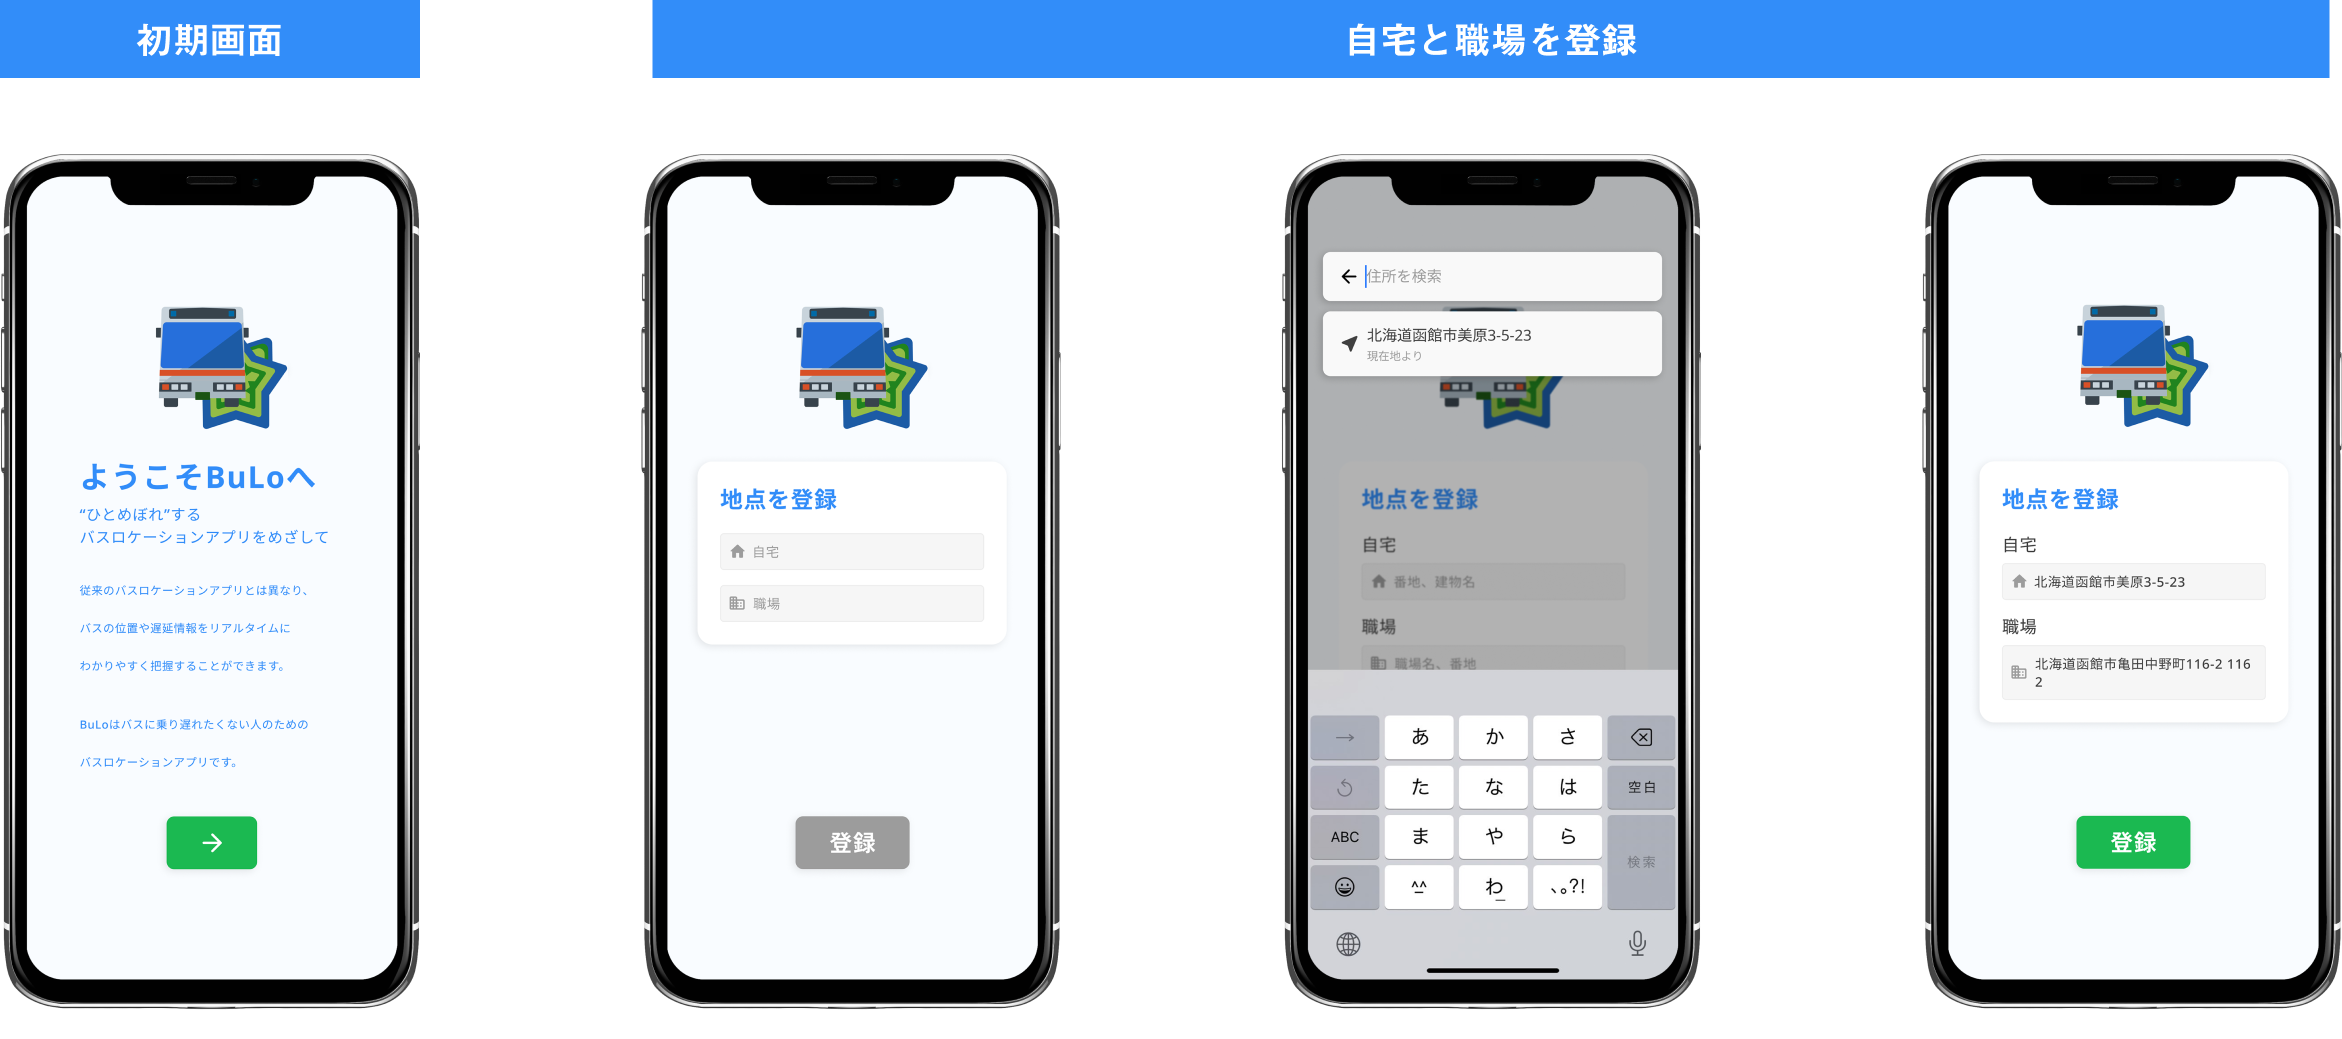
\includegraphics[width=14cm]{images/feature_register.png}
    \caption{住所を登録}
    \label{fig:feature_register}
\end{figure}
\subsection{Time-Distance ListとRoute View}
ユーザが住所を登録したあと,ユーザがアプリを開いた際は図\ref{fig:feature_td}の画面を表示する.
図\ref{fig:feature_td}の左側の画面は,後述するTime-Distance Viewの一覧である.
一覧は,バスがユーザの乗車するバス停に到着する順に表示される.
図\ref{fig:feature_td}の右側の画面は,各Time-Distance Viewをタップした際に表示される画面である.
ここではタップしたTime-Distance Viewと,ユーザとそのバスの現在地がマップ上に表示される.
\begin{figure}
    \centering
    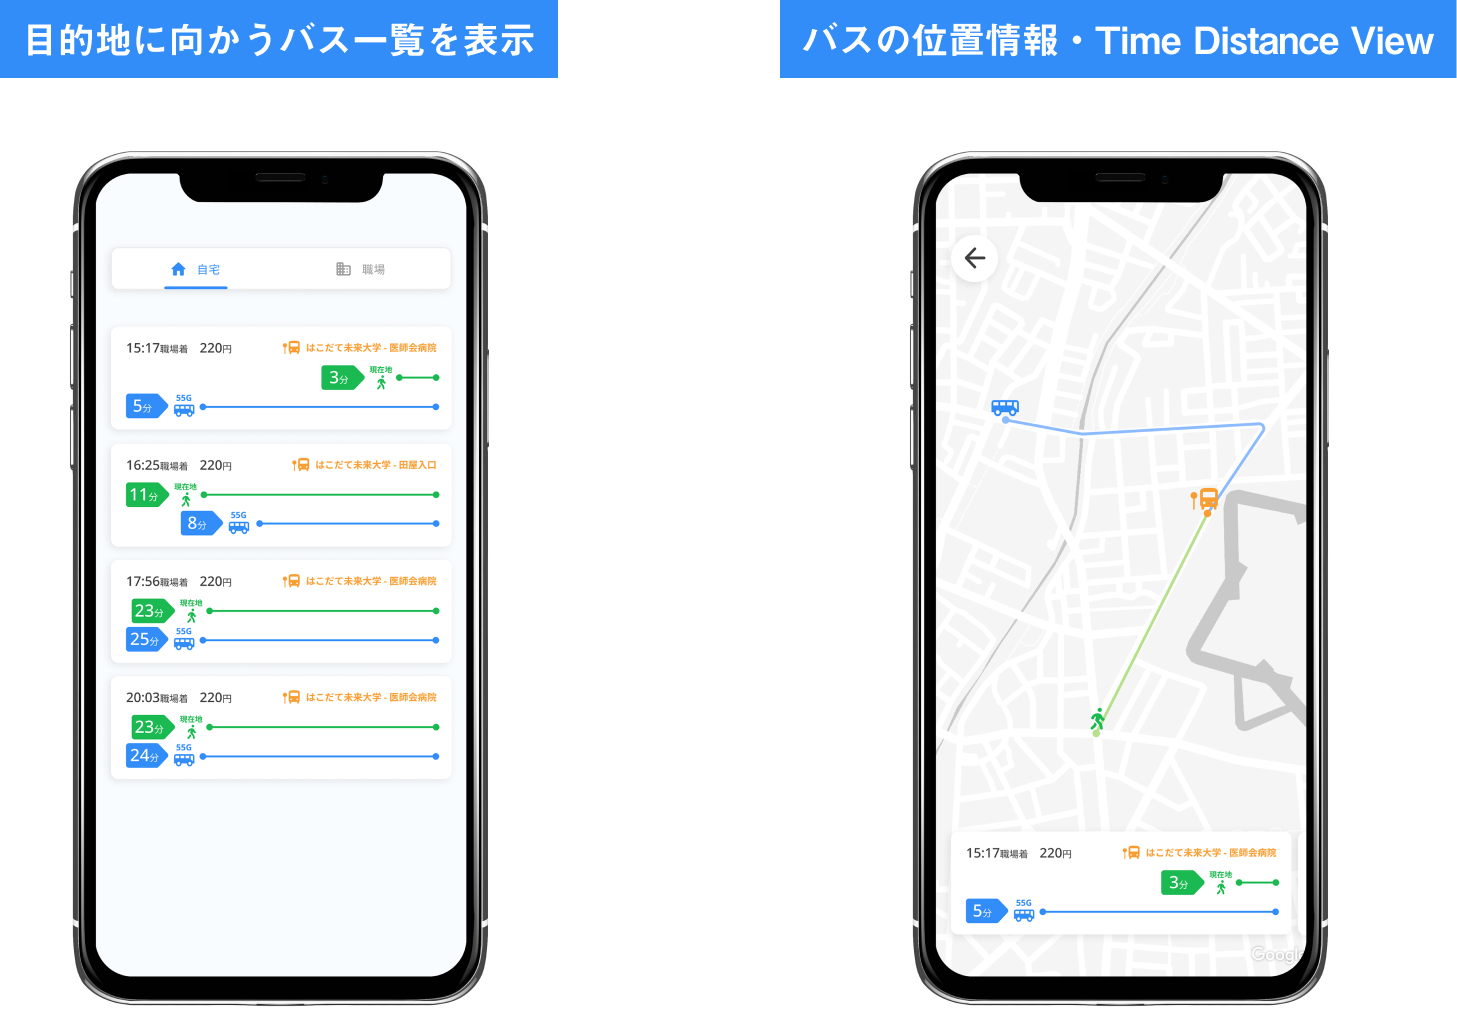
\includegraphics[width=14cm]{images/feature_td.png}
    \caption{Time-Distance ViewとRoute View}
    \label{fig:feature_td}
\end{figure}
\subsection{Time-Distance Viewの詳細}
Time-Distance Viewとは,ユーザの現在地・バスの現在地・バス停の3点を時間的グラフに表したものである.
これにより,ユーザは「バスに間に合うかどうか」,「バス停でどのくらい待つか」がひとめでわかる.
実装方法は図\ref{fig:feature_timedistanceview}に示す.
また,図\ref{fig:feature_timedistanceview}では以下の状況を考えている.
\begin{quote}
    \begin{itemize}
        \item ユーザの目的地は自宅(田屋入口の近く)
        \item 現在地からの最寄りのバス停ははこだて未来大学駅
        \item ユーザが乗るバスは55G
        \item ユーザが自宅に行くまでにかかる料金は220円
        \item バスは5分後にはこだて未来大学駅に到着する
        \item 現在地からはこだて未来大学駅まで徒歩で3分かかる
        \item 自宅には16:25に到着する
    \end{itemize}
\end{quote}
\begin{figure}
    \centering
    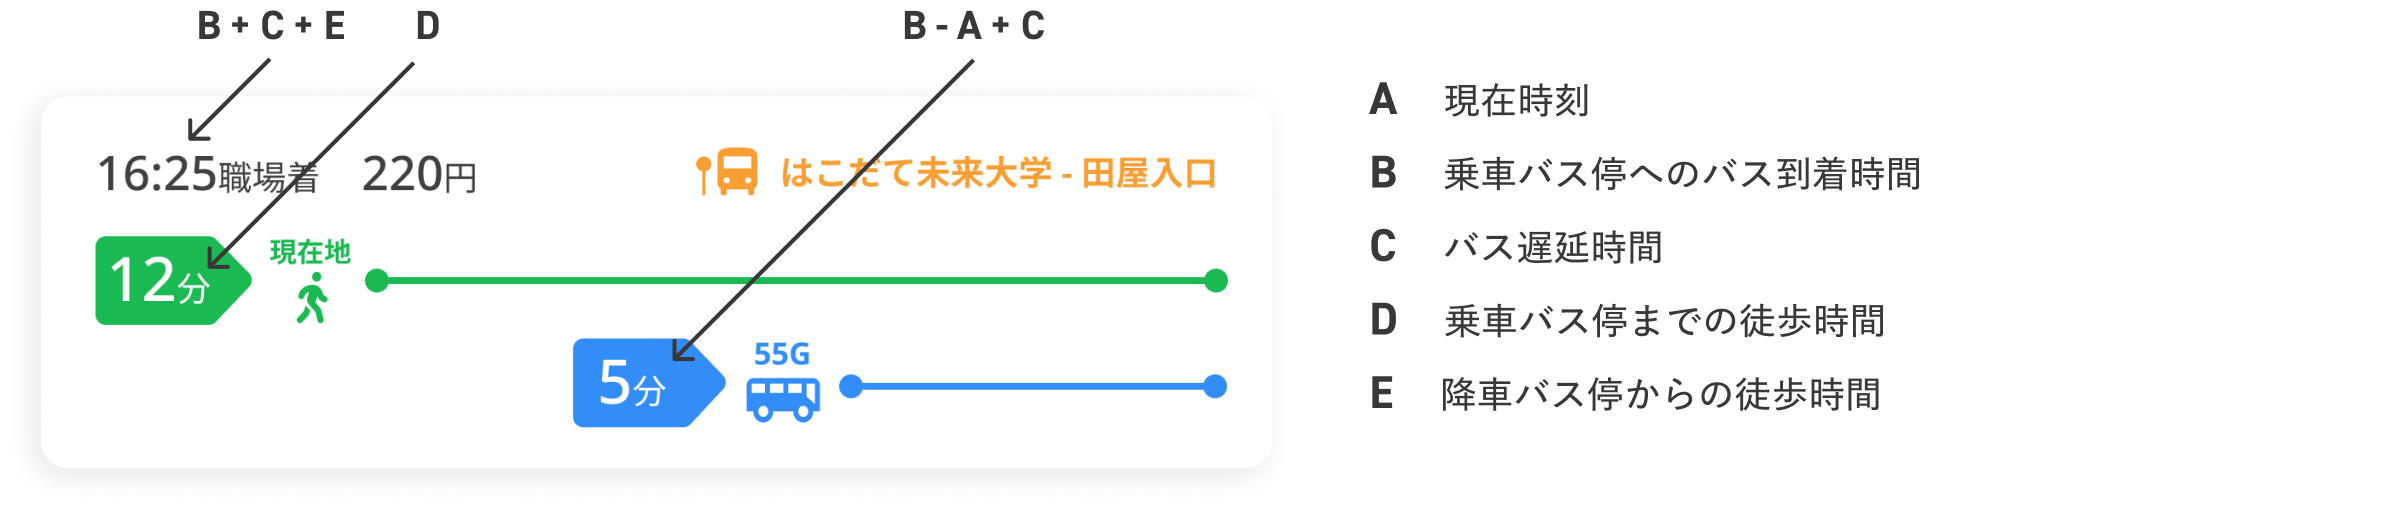
\includegraphics[width=14cm]{images/feature_timedistanceview.png}
    \caption{Time-Distance View}
    \label{fig:feature_timedistanceview}
\end{figure}
図\ref{fig:feature_timedistanceview2}では,想定されるTime-Distance Viewの例を示している.
図\ref{fig:feature_timedistanceview2}の左から,「ユーザがバスに安心して乗れる状態」
「ユーザがバス停でかなり待つことが予想できるため,バス停以外の場所で時間をつぶすことができる」
「ユーザよりバスの方が先にバス停に到着するが,走ることでバスに乗ることができる」状態である.
\begin{figure}
    \centering
    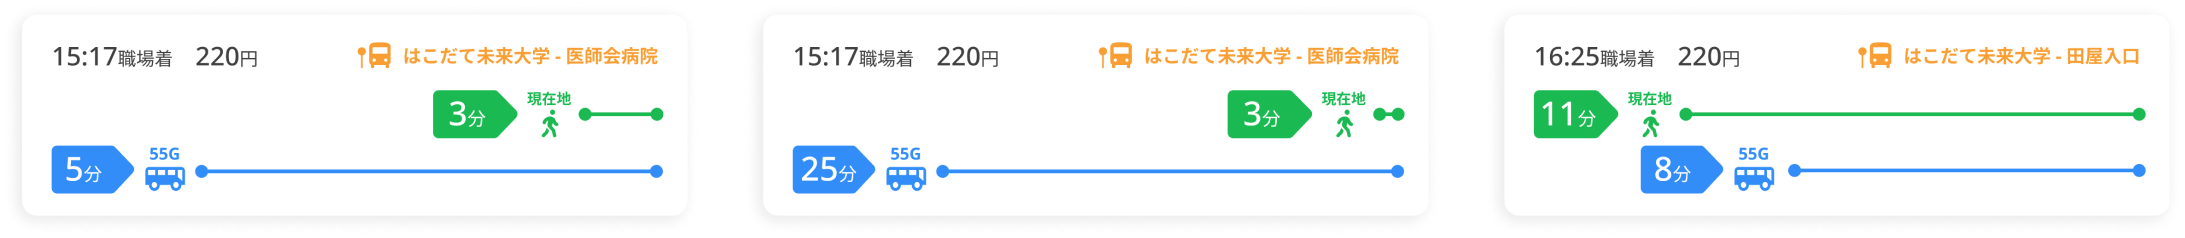
\includegraphics[width=14cm]{images/feature_timedistanceview2.png}
    \caption{Time-Distance Viewの例}
    \label{fig:feature_timedistanceview2}
\end{figure}
\bunseki{下村蒔里萌}

\section{デザインシステム}
本アプリは,簡潔で見やすく情報量の絞られたデザインを目指している.
アジャイル開発を行う上で,手戻りの少ない一貫性のあるUI改善を行うため,また,エンジニアとデザイナーの共通認識を図るために,
以下のデザインシステムを設定した.
\subsection{Colors}
本サービスのカラーパレットは図\ref{fig:feature_colors}のように設定した.
16進数のカラーコード(例:\#FF3B30)に具体的な値を与え使いやすくしたプリミティブトークン(例:red)と,
特定の用途別に定義したセマンティックトークン(例:alert)を定義している.
Figma上でのプロトタイプや実装では,セマンティックトークンを使用した.
\begin{figure}
    \centering
    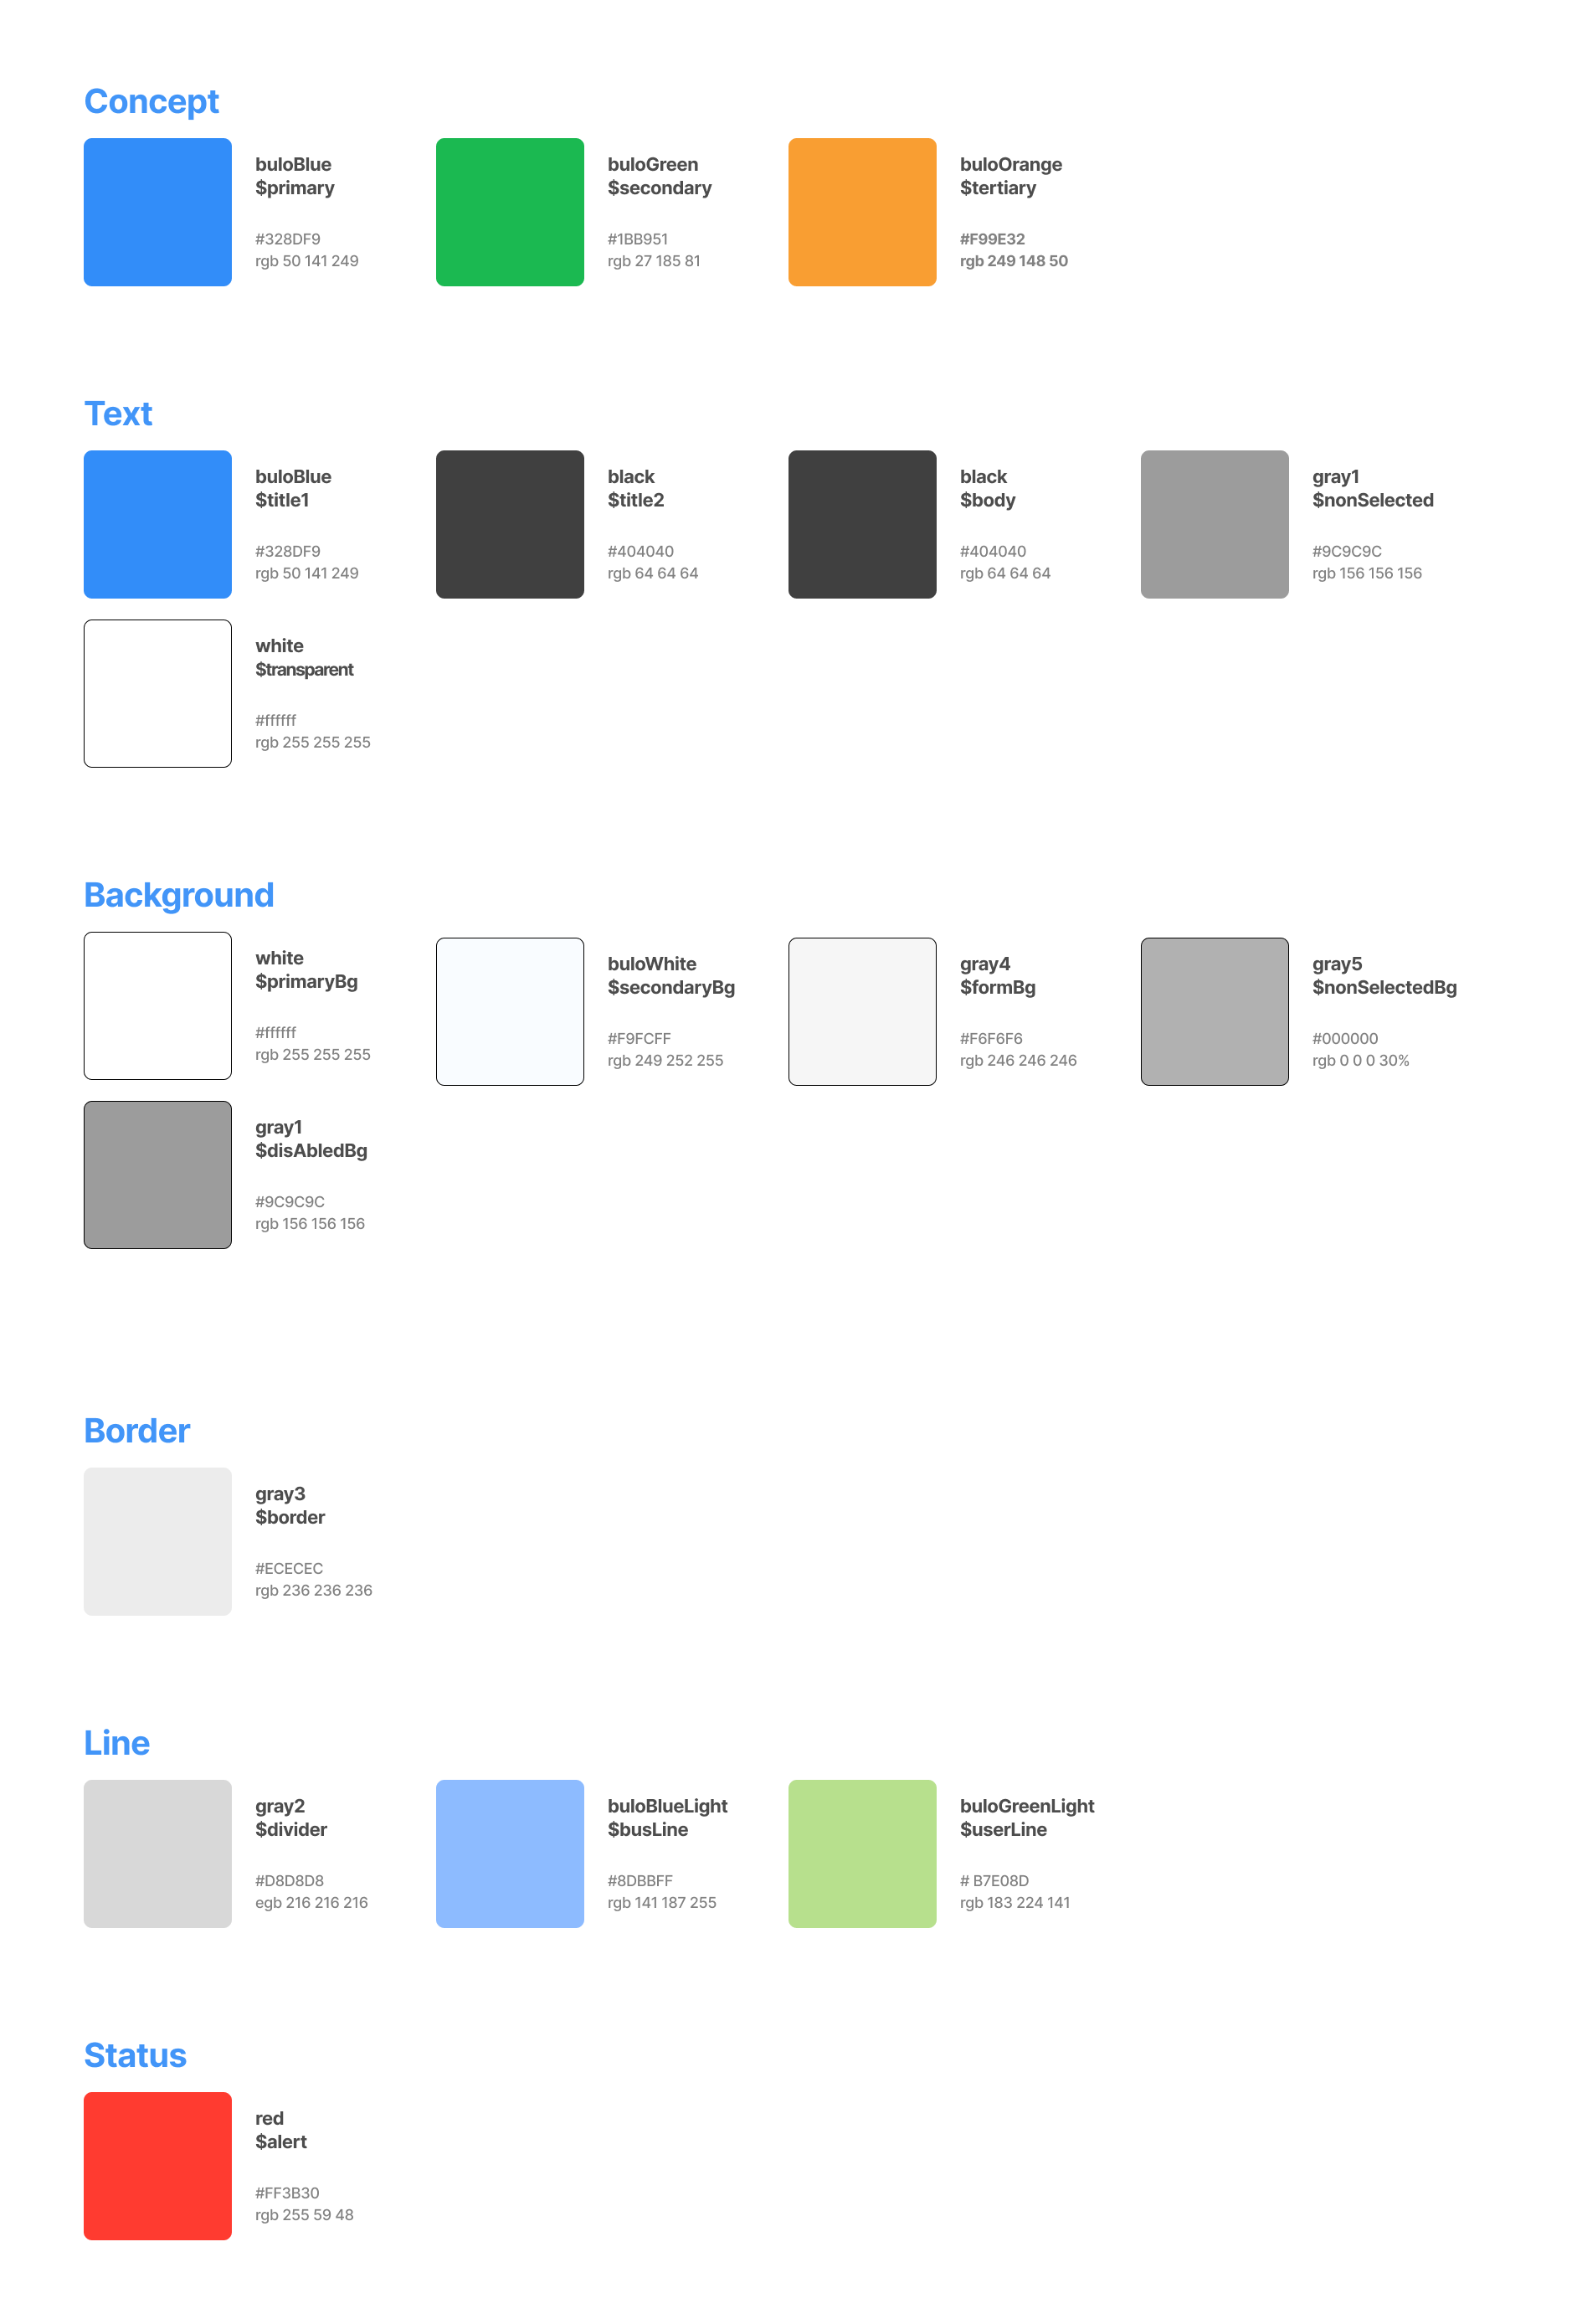
\includegraphics[width=10cm]{images/colors.png}
    \caption{デザインシステム Colors}
    \label{fig:feature_colors}
\end{figure}
\subsection{Typographies}
本サービスのフォントは図\ref{fig:typographies}のように設定した.
\begin{figure}
    \centering
    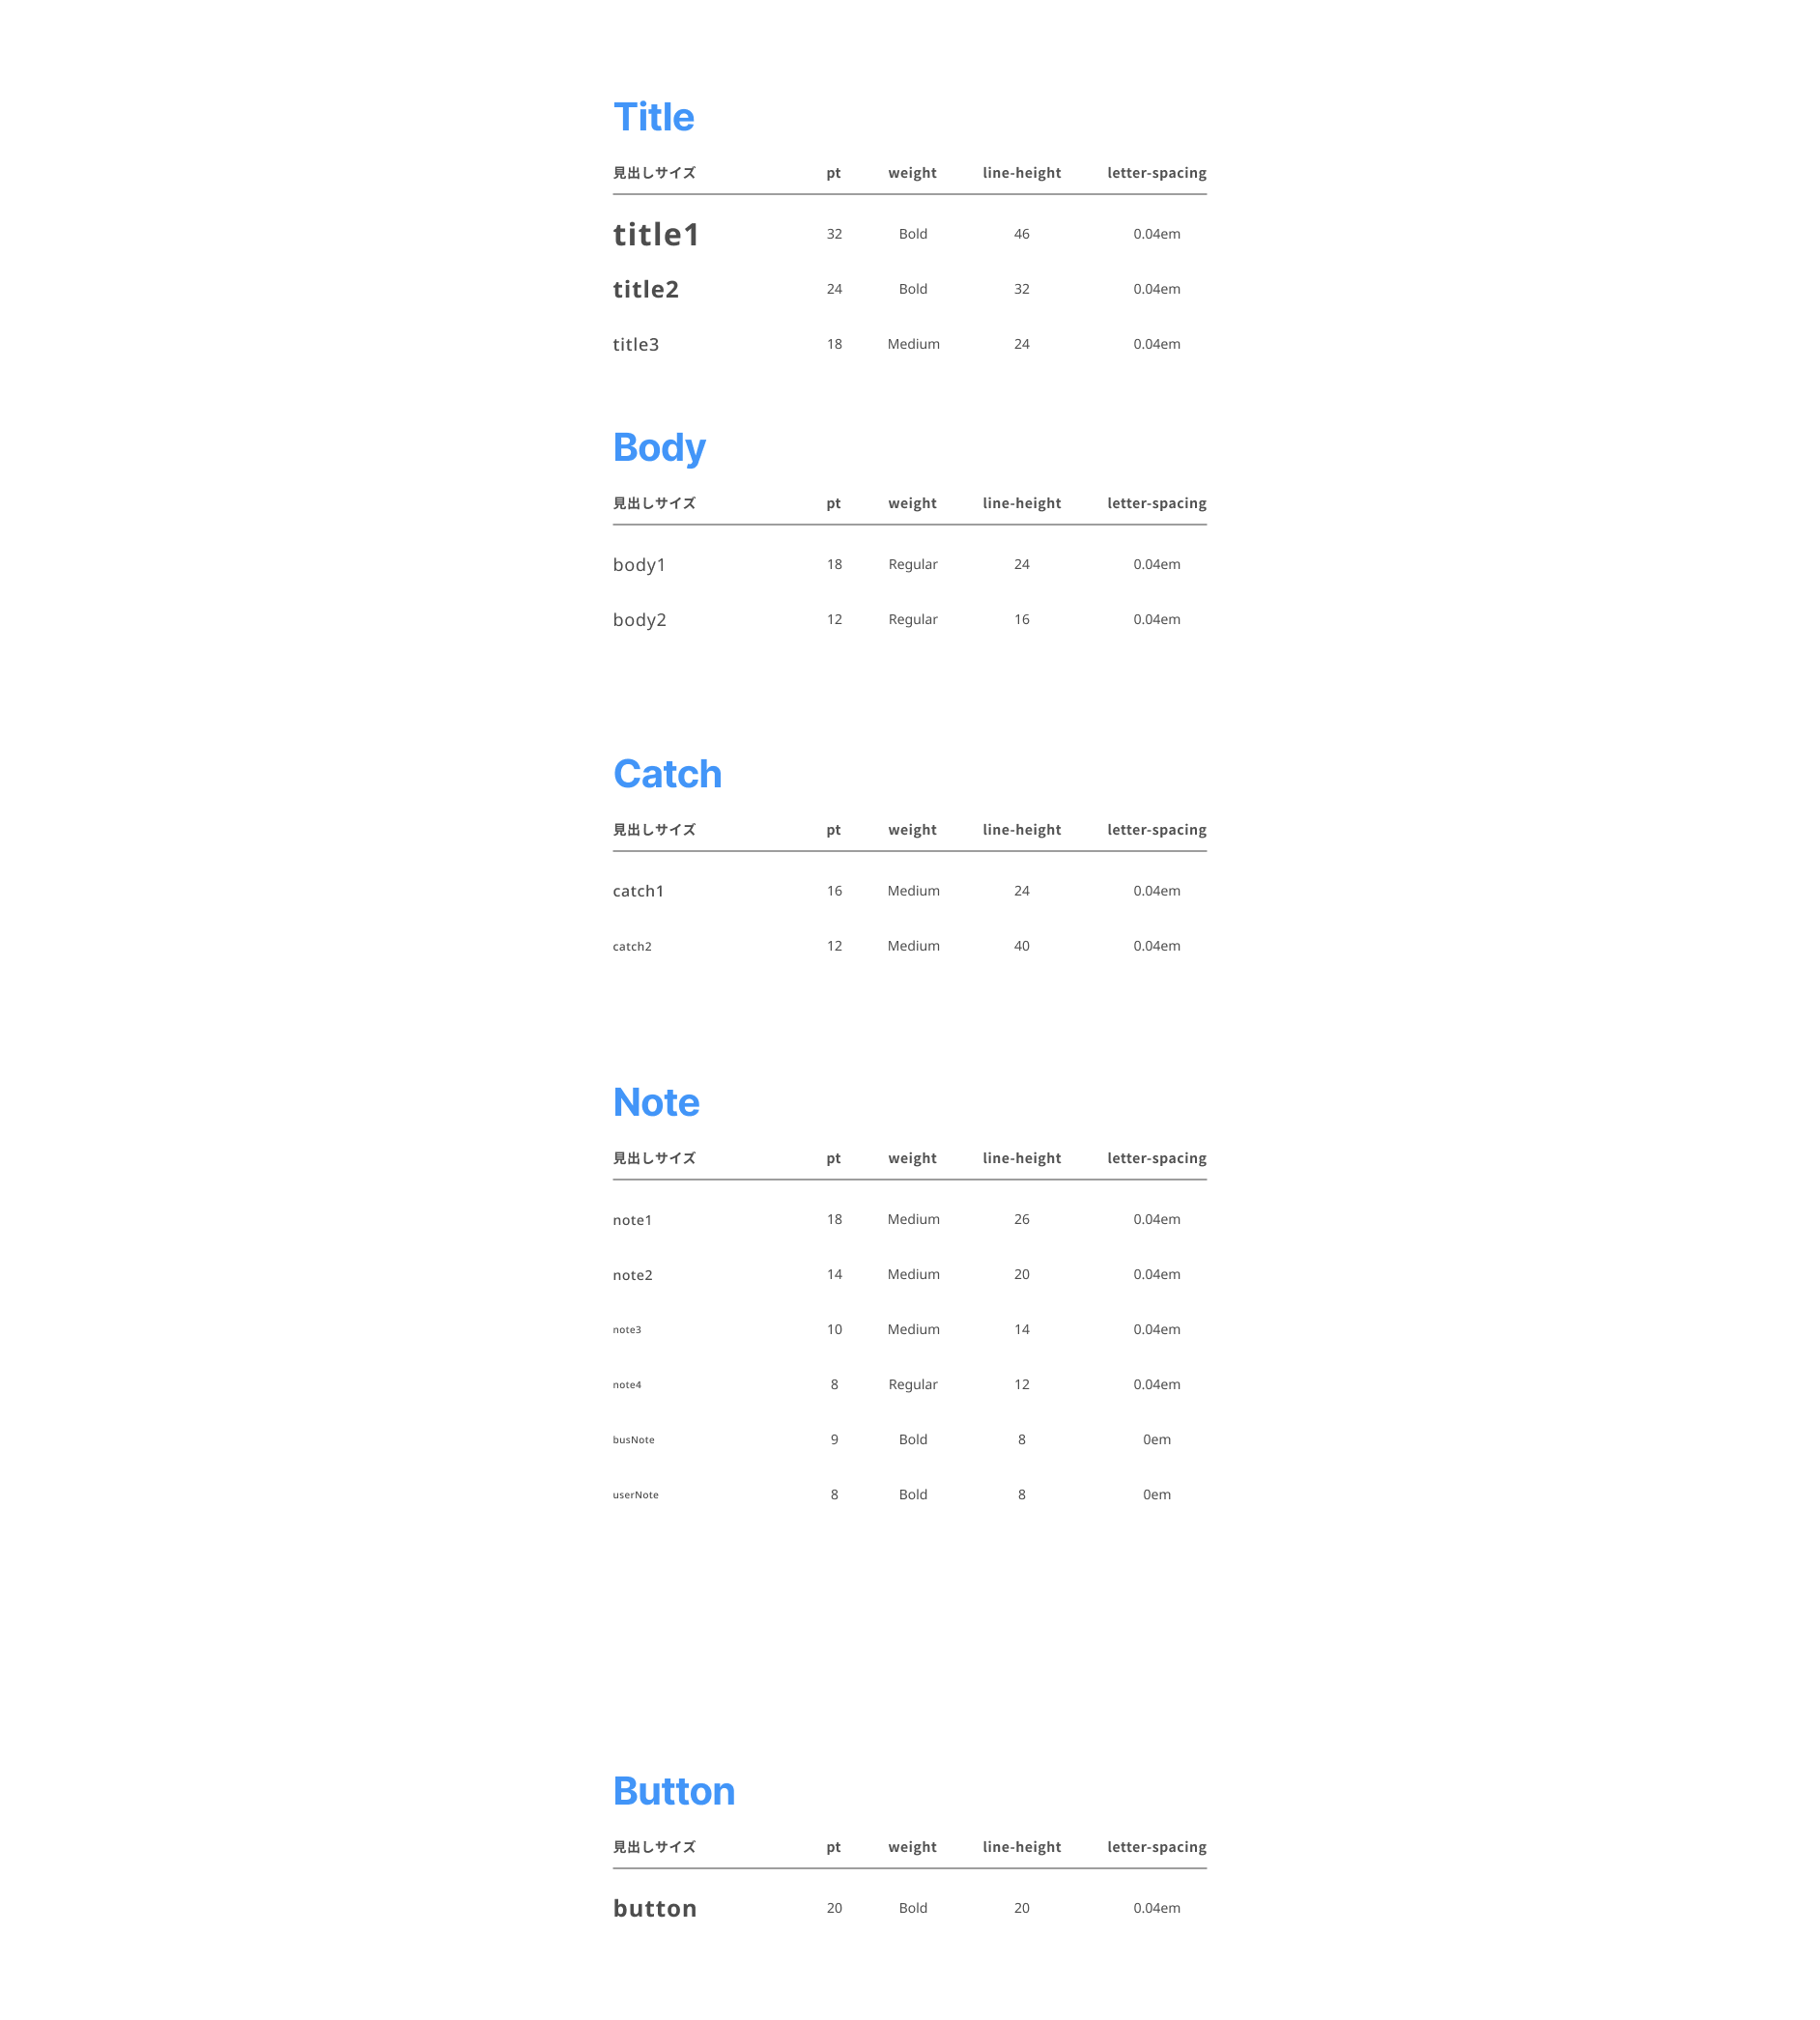
\includegraphics[width=10cm]{images/typographies.png}
    \caption{デザインシステム Typographies}
    \label{fig:typographies}
\end{figure}
\subsection{Icons}
    本サービスのアイコンは図\ref{fig:icons}のように設定した.
    主にMaterial Symbols and Icons\footnote{https://fonts.google.com/icons}を使用し,足りないものはPictogrammers\footnote{https://pictogrammers.com/}を使用した.
        \begin{figure}
            \centering
            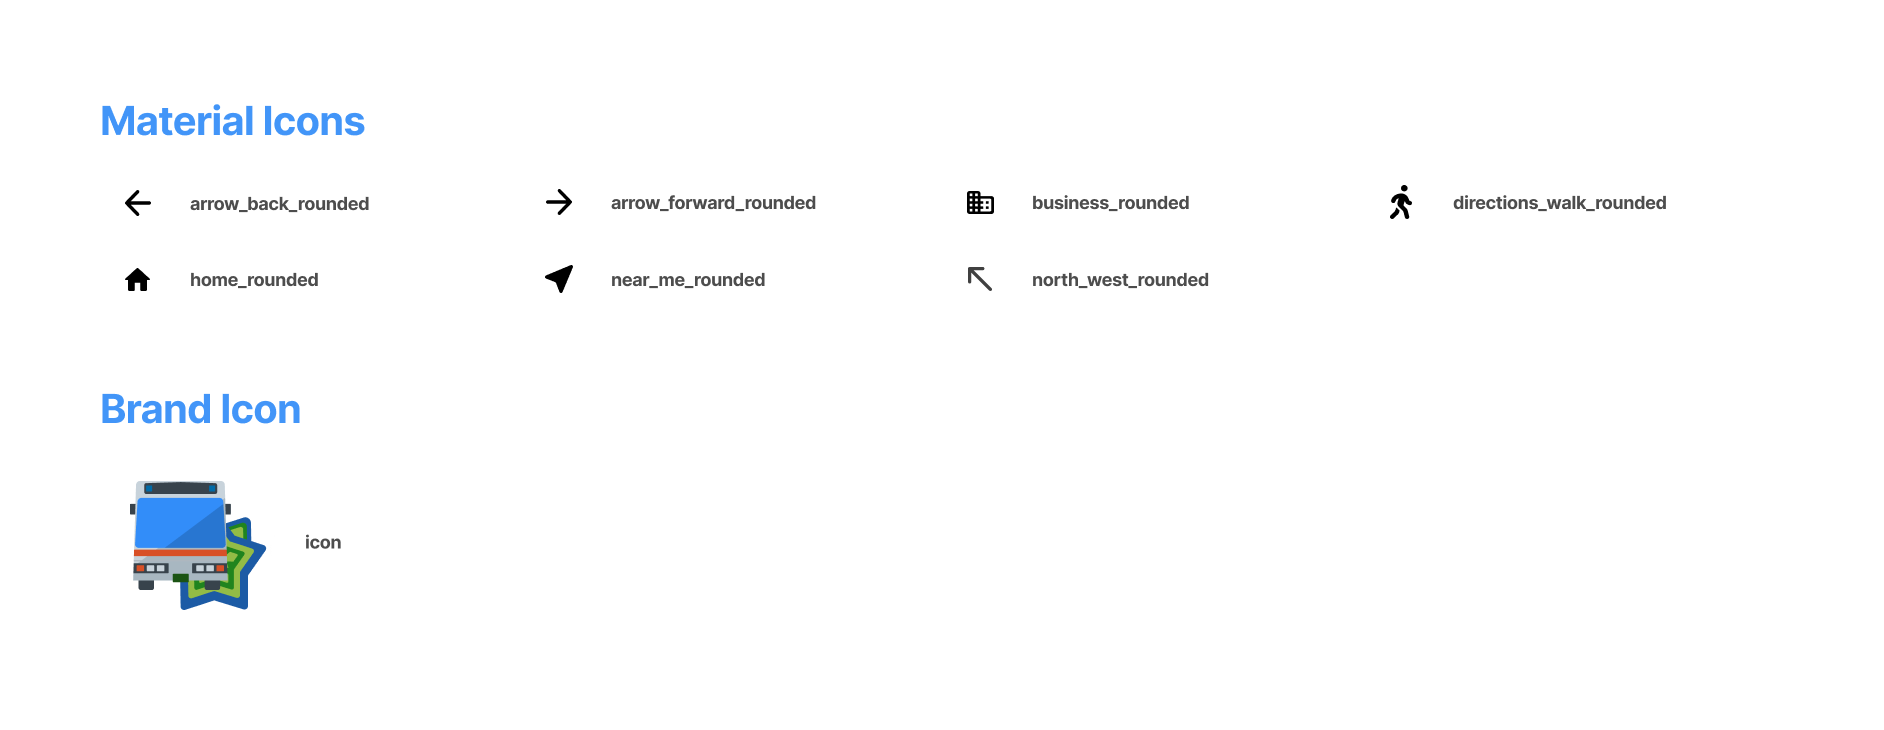
\includegraphics[width=10cm]{images/icons.png}
            \caption{デザインシステム Icons}
            \label{fig:icons}
        \end{figure}
\subsection{Shapes and Others}
    本サービスの形状とその他のデザインは図\ref{fig:shapes}のように設定した.
    ElevationやBlurは2つのレイヤー間のz軸上の深度を表す.
    インターフェイス上の最も上位の要素をより強調することで,アクションの重要度を伝える.
    Cornersは角丸を表し,4, 8, 16と3種類の数字を用意し,コンポーネントの短辺に合わせて角丸の数値を可変する.
    角丸を使用した図形の中に,角丸を使用した図形位がある場合は,
    外側の図形の角丸=内側の図形の角丸+内側の余白とする.
\begin{figure}
    \centering
    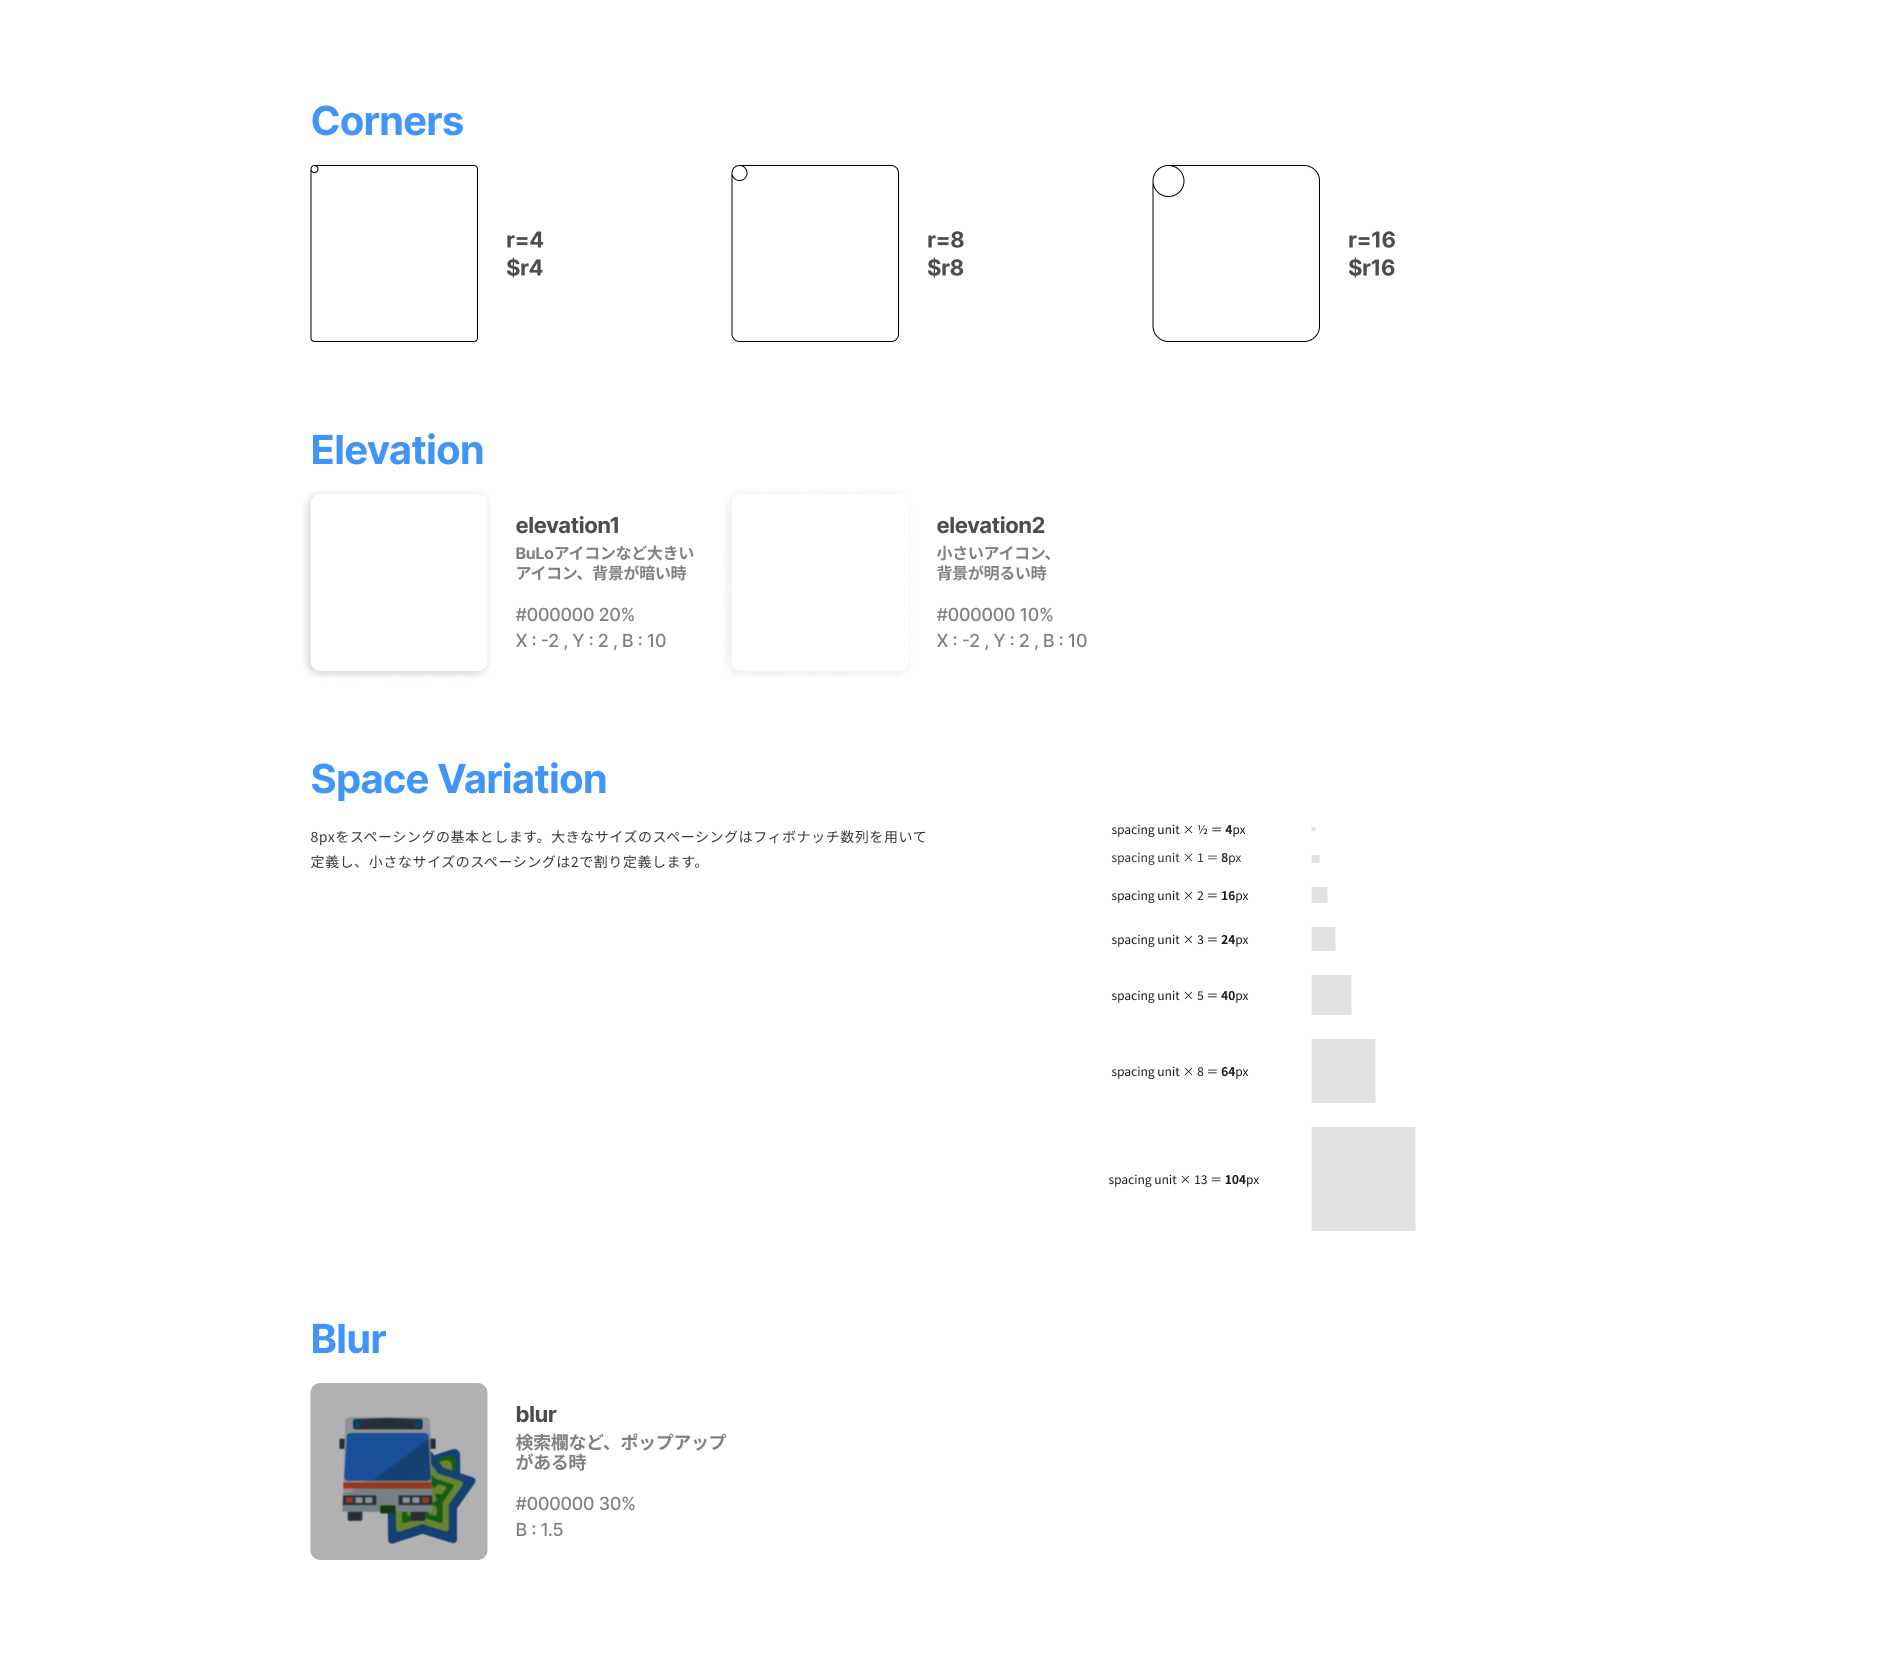
\includegraphics[width=10cm]{images/shapes.png}
    \caption{デザインシステム Shapes and Others}
    \label{fig:shapes}
\end{figure}
\bunseki{下村蒔里萌}

\section{システムの構成}
本サービスでは,マイクロサービスアーキテクチャを採用している.クライアントは,BFF (Backend for Frontend) を介して,バックエンドのマイクロサービスと通信する.
バックエンドのマイクロサービス間は,gRPCを用いて通信する.アーキテクチャ図を図\ref{fig:architecture}に示す.
\begin{figure}
    \centering
    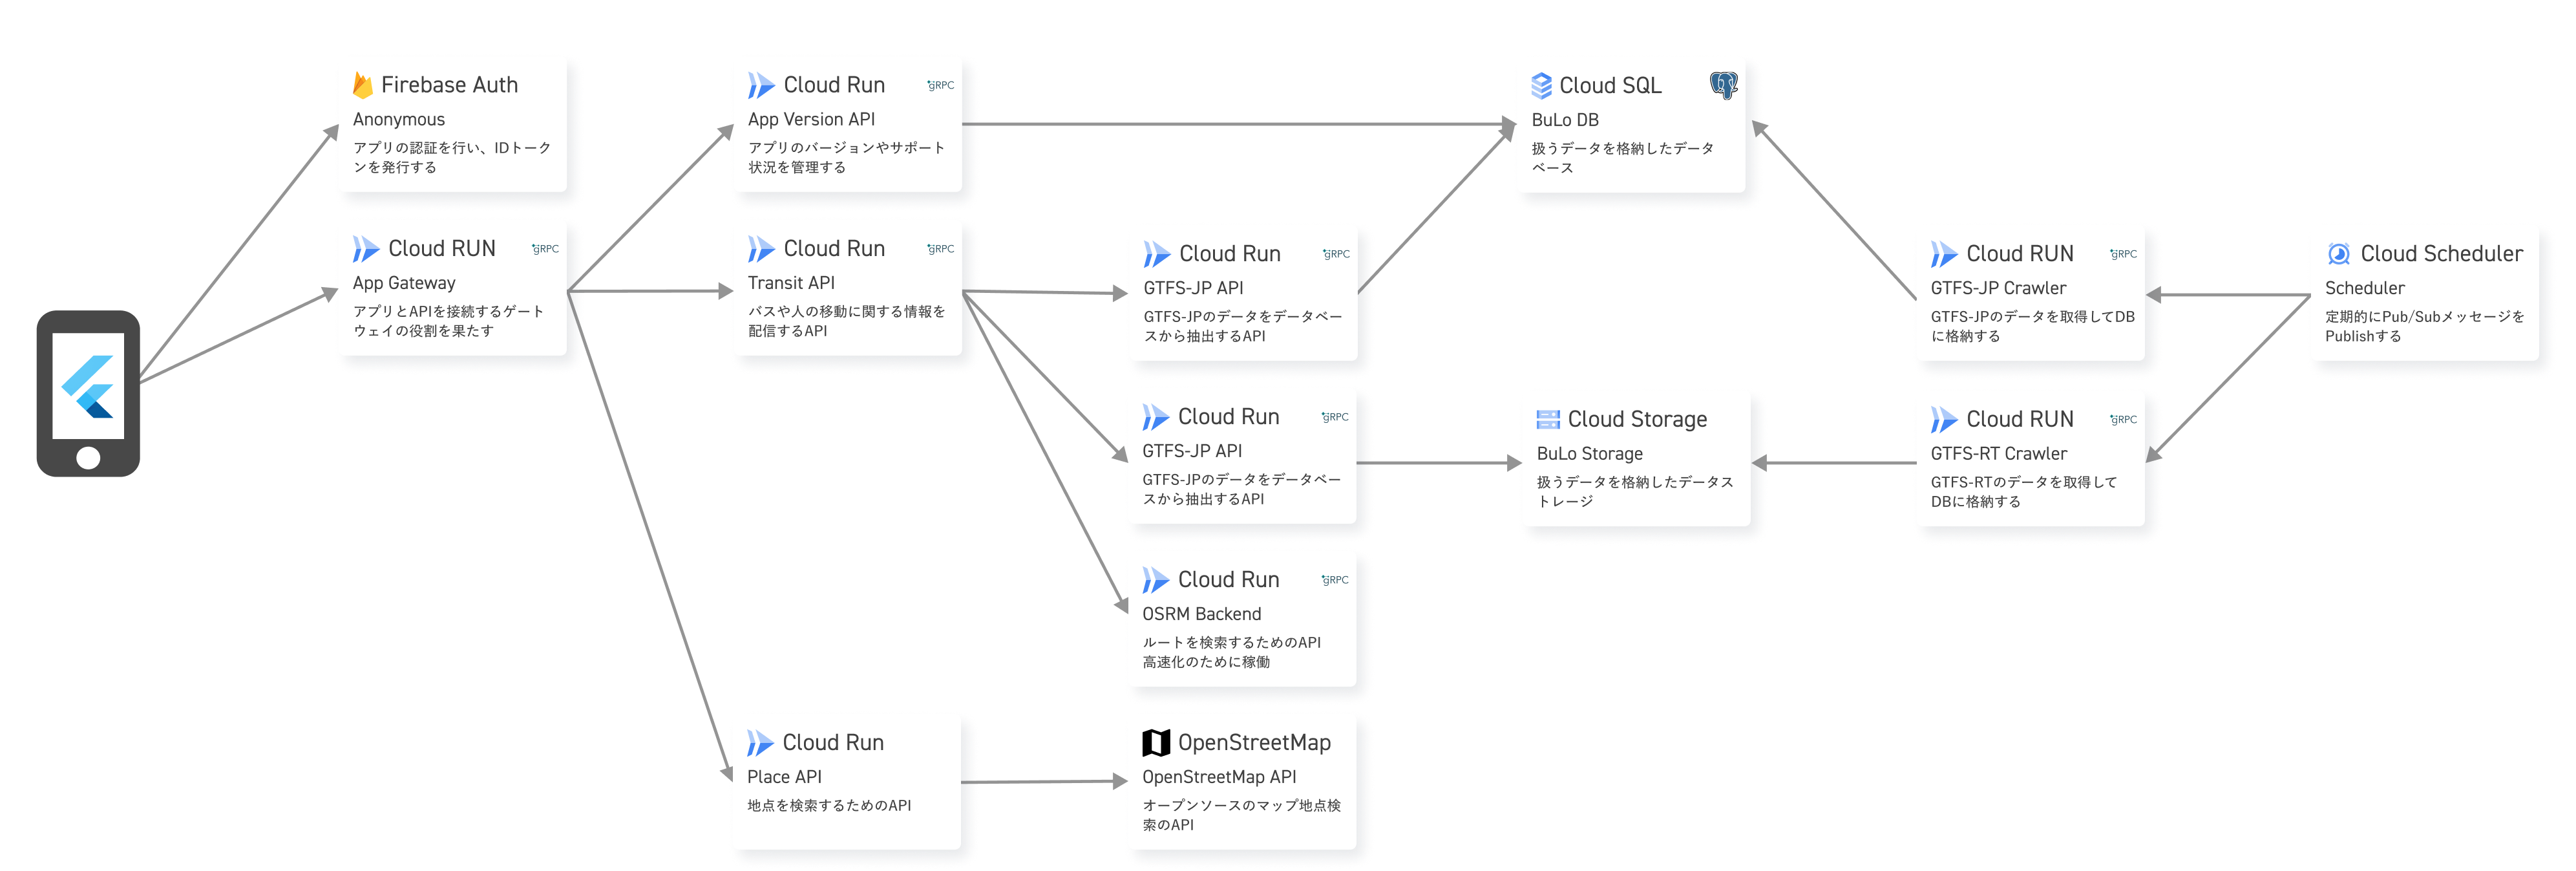
\includegraphics[width=14cm]{images/architecture_diagram.png}
    \caption{アーキテクチャ図}
    \label{fig:architecture}
\end{figure}
以下に,いくつかのマイクロサービスを抜粋して説明する.

\subsection{クライアントアプリケーション}
クライアントアプリケーションは,Flutter\footnote{https://flutter.dev/}を用いて開発した.Firebase Authentication\footnote{https://firebase.google.com/products/auth}を用いて,ユーザの匿名認証を行う.生成されたIDトークンを用いて,App Gatewayと通信をする.App Gatewayは,バックエンドのマイクロサービスと通信をして,クライアントが扱いやすい形で,データを返却する.高度なビジネスロジックをフロントエンド側で持たず,できる限りバックエンド側に切り出すようにした.

\subsection{Transit API}
本サービスで最も重要なマイクロサービスの一つである.クライアントアプリケーション内のTime-Distance ViewやRoute Viewを提供するために必要な情報を,GTFS-JPおよびGTFS-RTのデータから計算する.

\subsection{Place API}
地点を検索する際に,入力されたキーワードから,マッチする地点を検索するマイクロサービスである.検索には,OpenStreetMap\footnote{https://www.openstreetmap.org/}のデータからジオコーディングを行う,Nominatim\footnote{https://nominatim.org/}というオープンソースのジオコーディングツールを使用した.
\bunseki{及川寛太}

\section{使用した技術}
\subsection{Flutter}
当初は,iOSアプリをSwiftで,AndroidアプリをKotlinで開発する予定であったが,開発期間が短いことや人数が少ないことから,1つのコードベースで2つのプラットフォームをサポートできる,Flutterを採用した.

\subsection{GraphQL}
本サービスでは,当初,GraphQLサーバを介して,バックエンドのマイクロサービスと通信していた.
GraphQLのデメリットや,マイクロサービス間では,gRPCによる通信が行われていたことから,gRPCを用いて通信するように変更した.

\subsection{gRPC}
本サービスでは,マイクロサービス間通信,および,バックエンドのマイクロサービスとクライアント間通信にgRPCを用いている.

\subsection{PostgreSQL}
本サービスでは,GTFS-JPの静的データを保存し,各サービスからアクセスするために使用する.

\subsection{Google Cloud Platform}
本サービスの,データベースサーバはCloudSQL\footnote{https://cloud.google.com/sql/},バックエンドのマイクロサービスはCloud Run\footnote{https://cloud.google.com/run/}上で稼働している.
サーバレスサービスにより,サーバの管理にリソースを割くことなく,開発に集中することができる.
\bunseki{及川寛太}

\chapter{活動}
\section{ブレインストーミング}
各々が開発したいアイデアを,Miro\footnote{https://miro.com/}を使用して,書き出した.(図\ref{fig:brainstorm})
アイデアの例は以下である.

\begin{quote}
    \begin{itemize}
        \item 独り言を自動的に録音してテキスト化
        \item 健康促進アプリ(地図上でこれまで行った場所を塗りつぶす)
        \item 悩みがある人同士で会話できるもの
        \item 店など様々な場所の混雑度チェックアプリ
        \item 公共交通機関を携帯からリアルタイムに把握する
        \item 1日を可視化
    \end{itemize}
\end{quote}

各々違う色の付箋を使用し,KJ法を使用し意見をまとめた.
この活動ではさまざまな意見が挙げられたが,一番チームの共感を得たバス利用に関する問題について,今後の活動を絞った.

\begin{figure}[H]
    \centering
    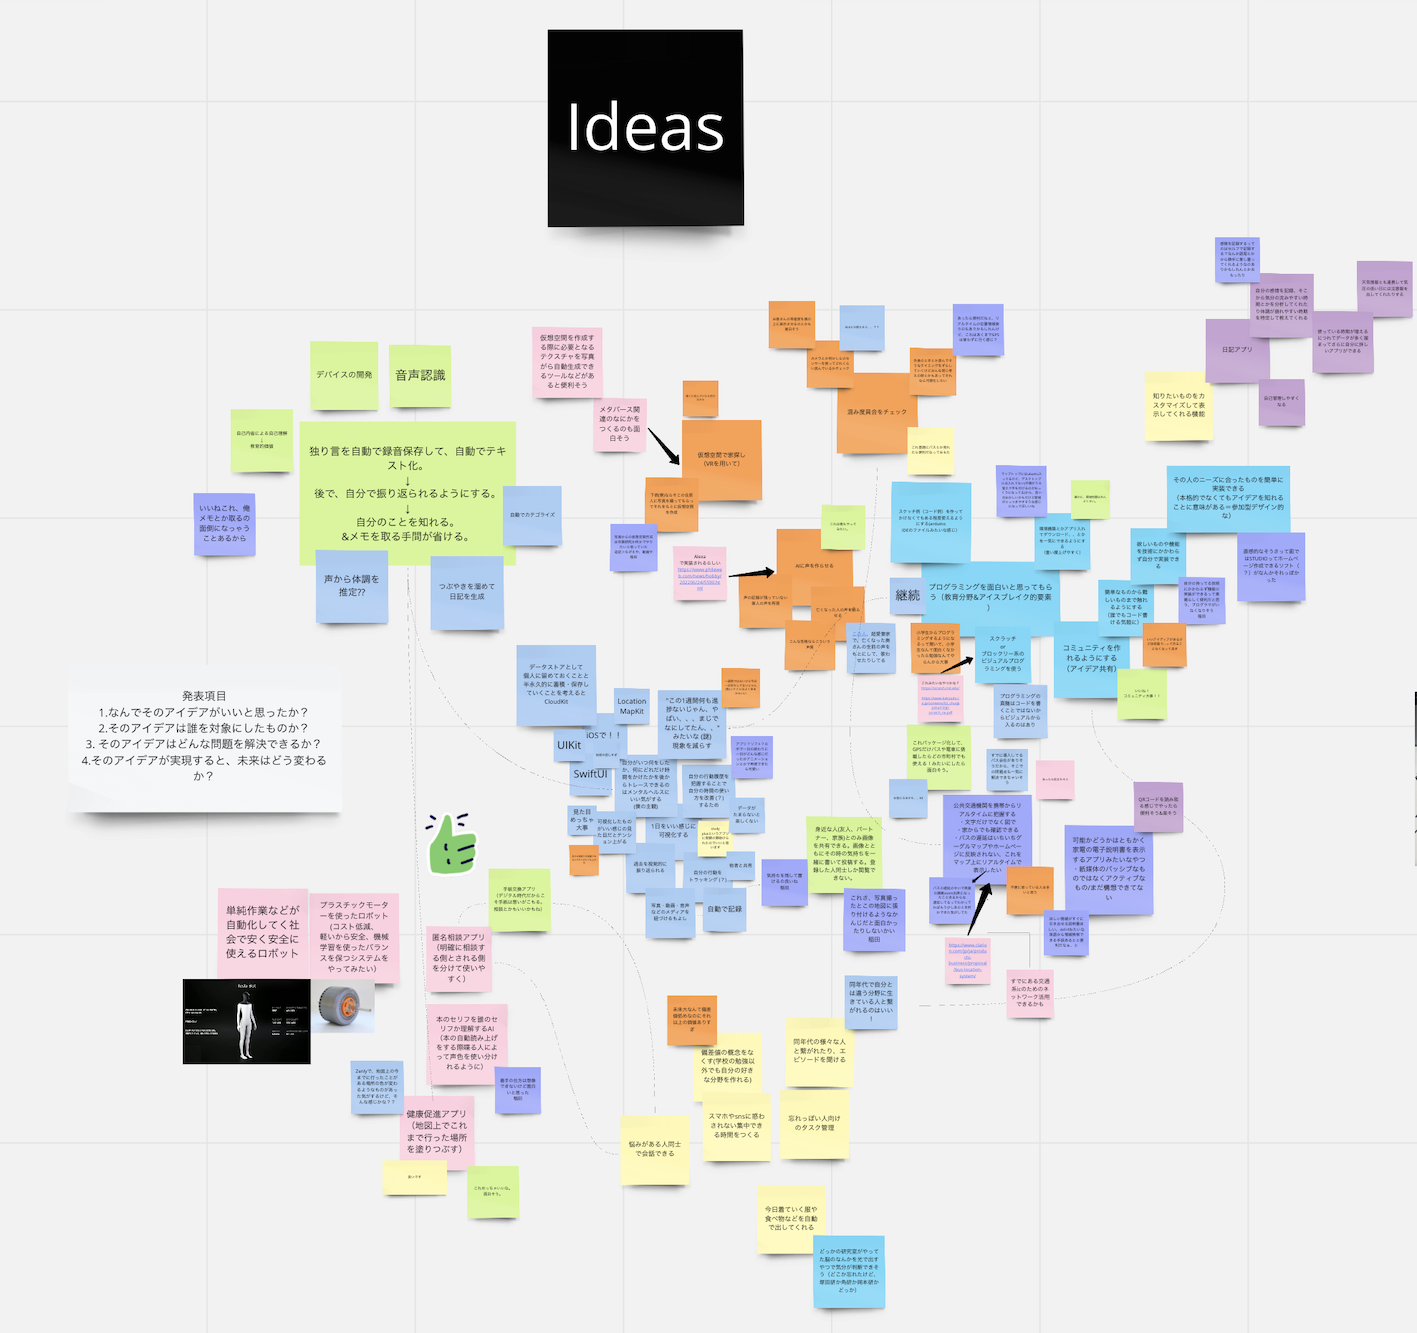
\includegraphics[width=9cm]{images/brainstorm.png}
    \caption{ブレインストーミング}
    \label{fig:brainstorm}
\end{figure}
\bunseki{大津武琉}

\section{アイデアの深掘り}
上記のブレインストーミングで挙げられたアイディアは煩雑なものであったため,実際に我々がバスを利用してきた中で不便に感じたことを考え,
解決策への仮説を列挙した.以下はその例である.

\begin{quote}
    \begin{itemize}
        \item 交通系ICカードを取り込み残高を表示
        \item バス停までの徒歩時間表示
        \item バスの時刻表表示
        \item 地図上に表示するバスの数を変えることができる
    \end{itemize}
\end{quote}

\begin{figure}[H]
    \centering
    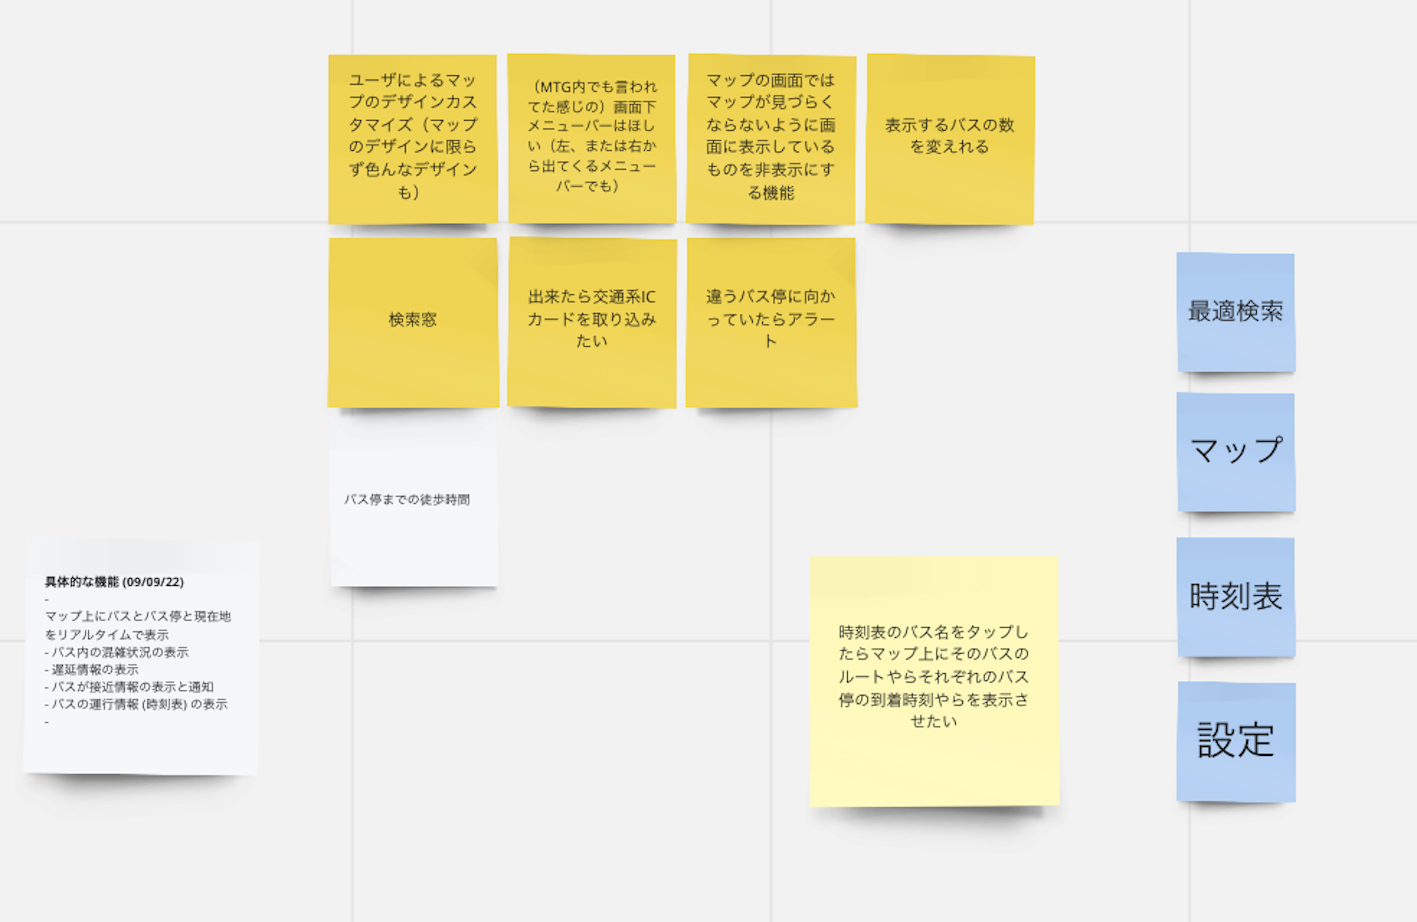
\includegraphics[width=14cm]{images/dig.png}
    \caption{アイデアの深掘り}
    \label{fig:dig}
\end{figure}
\bunseki{下村蒔里萌}

\section{アプリ名の決定}
各々が本サービスのコンセプトから考えられるサービス名を考えた.以下はその例である.
\begin{quote}
    \begin{itemize}
        \item BuLo (ブーロ) : BusとLocationの頭をとったもので,美しく (Beautiful) ,有用なユーザーインターフェースUseful (UserInterface) を持つライブ (Live) で最良のオプション (Option) である.バスロケーションシステムという意味も持つ.
        \item Loco (ロコ) :「ロケーション」と「どこ」をかけたもの.
        \item nuts (ナッツ) : No trouble with busの各単語から1文字とって組み合わせたもの.
        \item バスらく: バスをらくに使えるアプリを略したもの.横文字のアプリ名がたくさんあるが,ぱっと思い出しにくいため,名前からすぐにどんな用途かわかるものを提案した.
        \item ばすけん: バス検索を省略したもの.
    \end{itemize}
\end{quote}
上記のものでメンバ内で多数決をとった結果,BuLo (ブーロ) という名前に決定した.
BuLoはBus Locationの頭をとったものであり,
美しく (Beautiful) ,有用なユーザーインターフェースUseful (UserInterface) を持つライブ (Live) で最良のオプション (Option) であるバスロケーションシステムという意味も持つ.
\bunseki{下村蒔里萌}

\section{開発プラットフォームの決定}
まず,iOSとAndroidの2プラットフォームのネイティブアプリを並行して開発するか,クロスプラットフォームのネイティブアプリを開発するか,ということについて考えた.
本グループでは2つの理由からクロスプラットフォーム開発に決定した.
1つ目の理由は,グループの規模が小さいことである.プラットフォームを分けると,各プラットフォーム2〜3人となってしまい各人の負担が大きい.
2つ目の理由は,本グループ全体の技術力が少ないことである.
本グループには,過去に開発者としてアプリケーション開発を行ったことのある者が1人しかいない.
ほかのメンバは経験がなく,1から学習を始めるため,学習コストが大きい.
以上の理由より,クロスプラットフォームのネイティブアプリの開発を進める形となった.
使用するフレームワークはクロスプラットフォームの代表例であるFlutter\footnote{https://flutter.dev/}となった.
\bunseki{及川寛太}

\section{メンバの役割決定}
本グループでは4人のメンバで行っている.各メンバの役割については以下の通りである.

\subsection{プロダクトオーナー}
プロダクトオーナーはプロダクトの責任者であり,開発チームを活用して,そのプロダクトが生み出す価値を最大化する責任がある\cite{scrum}.
\begin{quote}
    \begin{itemize}
        \item 及川 寛太
    \end{itemize}
\end{quote}

\subsection{スクラムマスター}
スクラム開発を円滑に進める役割がある.
具体的に,アジャイルとスクラムの価値を維持し,ほかの人がスクラムを理解し実践するのを助ける,スクラムのミーティングをファシリテートする \cite{scrum_master}.
\begin{quote}
    \begin{itemize}
        \item 大津 武琉
    \end{itemize}
\end{quote}

\subsection{デザイナー}
問題やユーザ像の分析より,アプリのUXやUIを考え,Figma\footnote{https://www.figma.com/}でプロトタイプを作成する.
実際にプログラムを書く際に必要な,レスポンシブな数値などのデザインシステムを作成する.
\begin{quote}
    \begin{itemize}
        \item 下村 蒔里萌
    \end{itemize}
\end{quote}

\subsection{iOSアプリ}
クロスプラットフォーム開発を行うが,iOS独自の開発が必要な場合や問題が発生した場合に,優先的に対応にあたる.
\begin{quote}
    \begin{itemize}
        \item 及川 寛太
        \item 下村 蒔里萌
    \end{itemize}
\end{quote}

\subsection{Androidアプリ}
クロスプラットフォーム開発を行うが,Android独自の開発が必要な場合や問題が発生した場合に,優先的に対応にあたる.
\begin{quote}
    \begin{itemize}
        \item 大津 武琉
        \item 稲田敬介
    \end{itemize}
\end{quote}

\subsection{サーバサイドエンジニア}
バスの運行に関わるデータの収集・記録・管理を行う.また,クライアント側が必要とする情報を素早く提供するシステムを開発する.
\begin{quote}
    \begin{itemize}
        \item 及川 寛太
        \item 大津 武琉
    \end{itemize}
\end{quote}
\bunseki{稲田敬介}

\section{Git・GitHubの習得}
チーム開発を進める中で必要不可欠であるバージョン管理アプリのGitHub\footnote{https://github.com/}の勉強会を行なった.メンバの過半数がGitHubを触ったことがなかったため,使用経験がある人から基本的な使用方法を教えてもらい,実際にGit\footnote{https://git-scm.com/}の機能であるClone,Commit,Push,Fetch,Merge,Pullを行なってGitHubについて学んだ.
\bunseki{稲田敬介}

\section{プロトタイプの作成}
\subsection{プロトタイプver.1}
アプリのプロトタイプをFigma\footnote{https://www.figma.com/}を用いて作成した (図\ref{fig:prototype_v1}) .
左から1枚目の画面は自分の現在地を表示させている.
2〜4枚目は目的地を入力する画面となっている.
5〜6枚目は現在地から2〜3枚目で入力した場所までのバスを表示させる.
7枚目では5〜6枚目で選択したバスと自分との位置関係をグラフと地図で表示させる.

\begin{figure}[H]
    \centering
    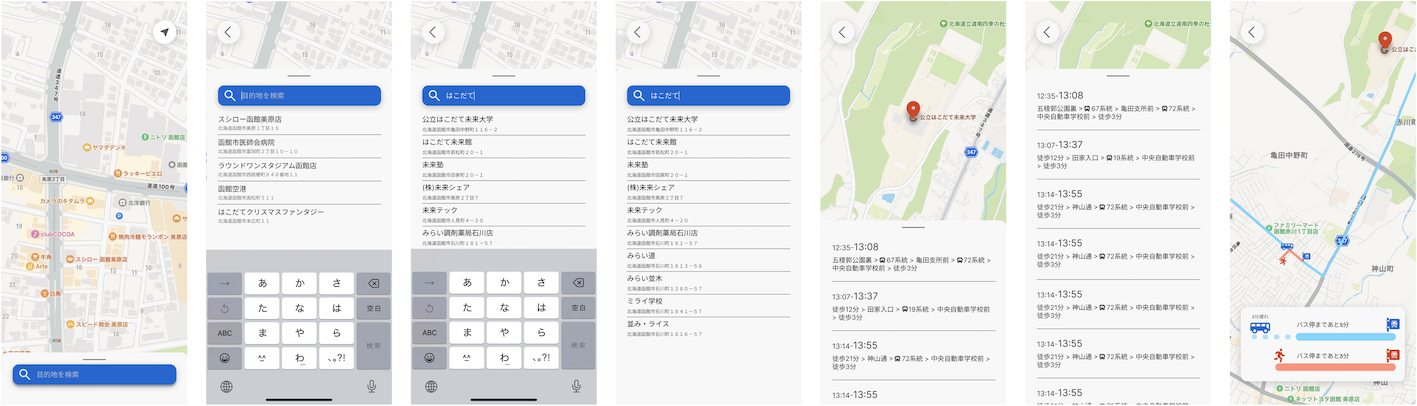
\includegraphics[width=14cm]{images/prototype_v1.png}
    \caption{プロトタイプver.1}
    \label{fig:prototype_v1}
\end{figure}

\subsection{フィードバック}
実際にプロジェクトメンバにFigma\footnote{https://www.figma.com/}で作成した図\ref{fig:prototype_v1}のプロトタイプを使用してもらった.
その際たくさんの質問,指摘,意見をいただいた.一番右の画面に対して,「下のバスと人との位置関係のグラフはいるのか?」,
「現在動いているバスの位置情報と自分の位置情報が分かれば大体どれくらいにバス停にいけばいいのかわかるのでは?」という意見をいただいた.
それらの意見に対し,ターゲットユーザを絞ることとした.

実際に得たフィードバックから,ターゲットユーザが定まっておらず,このアプリは何のため,誰のためのアプリなのかがわからないことに気がついた.
そこでチームでもう一度ターゲットユーザについて話し合い以下のように確立させた.

\begin{quote}
    \begin{itemize}
        \item 通勤通学にバスを使っていて,バスの乗降地点が毎回同じ
        \item バスに乗り遅れたくない
        \item バス停で待ちたくない
        \item 10代後半から20代前半
    \end{itemize}
\end{quote}

\subsection{プロトタイプver.2}
確立させたターゲットユーザに合う機能のみを実装するとしたため,合わせてプロトタイプを改善した.

図\ref{fig:prototype_v1}のプロトタイプではユーザが毎回移動先・移動元を検索していたが,
最初に登録をすることで,検索を毎回行う工程を省いた.通勤通学など,使用するバスが決まっているというユーザ像には,
地点の検索は無駄な工程であった.

アプリ全体のデザインとしては,色やアイコンを改善した.
具体的には,Time-Distace Viewのアイコンとその色を変更した.以前は人のアイコンが走っている人間のアイコンであり,
赤色を使用していたため,焦りを与えていた.そのため,色を改善し,さらに同レベルの情報の色のコントラストを揃えた.
また,Flutter\footnote{https://flutter.dev/}で開発をするにおいて,アイコンをMaterial Design\footnote{https://m3.material.io/}に統一した.

Time-Distance Viewについて,どの駅を使用するのか,何円かかるか,何時に到着するかなどの,ユーザが必要最低限と感じる情報を追加した.
さらに,ウィジェット全体のサイズやレイアウトを改善した.

最後に,アプリを開いた時にランディング画面を設けることで,アプリ全体の概要や印象をユーザがわかりやすくなるよう改善した.

\begin{figure}[H]
    \centering
    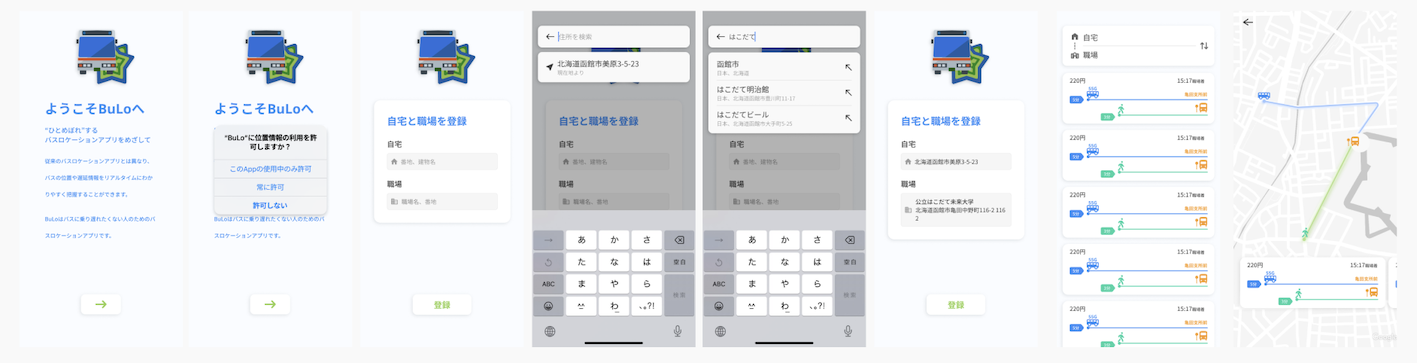
\includegraphics[width=14cm]{images/prototype_v2.png}
    \caption{プロトタイプver.2}
    \label{fig:prototype_v2}
\end{figure}

\subsection{フィードバック}
後述する中間発表会にて,プロトタイプver.2についてのフィードバックをいただいた.
その際たくさんの質問,指摘,意見をいただいた.
図\ref{fig:prototype_v2}の左から7,8枚目の画面に対して,「グラフの右端がバス停であることがわかりづらい」,
左から1〜3枚目の画面に対して,「登録ボタンの視認性が悪い」という意見をいただいた.

\subsection{プロトタイプver.3}
図\ref{fig:prototype_v3}の左から1〜3枚目の画面は初期画面である.
4〜6枚目は目的地を入力する画面となっている.
7枚目は現在地から4〜3枚目で入力した場所までのバスを表示させる.
8枚目では4〜6枚目で選択したバスと自分との位置関係をグラフと地図で表示させる.
図\ref{fig:prototype_v2}へのフィードバックをもとに,バスと現在地の時間的なグラフを改善した.
また,図\ref{fig:prototype_v3}の左から4〜6枚目の画面,すなわち目的地入力画面では,登録ボタンの視認性を向上させた.

\begin{figure}[H]
    \centering
    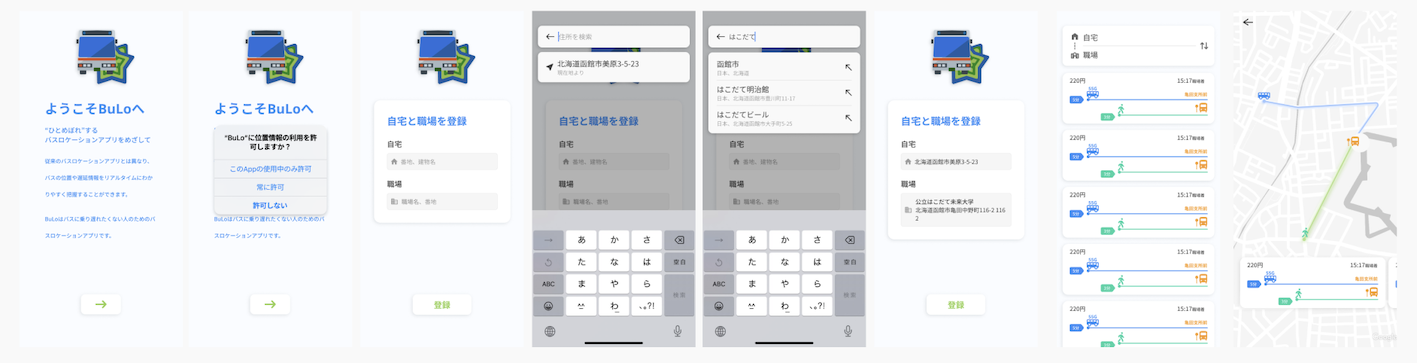
\includegraphics[width=14cm]{images/prototype_v3.png}
    \caption{プロトタイプver.3}
    \label{fig:prototype_v3}
\end{figure}
\bunseki{下村蒔里萌}

\section{リスク分析}
プロジェクトを行ううえでリスクは必ず存在する.そのため,リスクに関して対策を講じておくことが必要である.
我々は,リスクマネジメント\cite{risk}と題して,リスクに対して起こりうる被害の大きさや,どのように対策するのか等を考えた.
まず初めにプロジェクトメンバを3グループに分け,それぞれのチームでメンバが持ち寄った起こりそうなリスクをまとめた.
その後それぞれのリスクに対して,そのリスクが被る被害,発生確率,影響度,脅威,対策を考えた.
脅威については発生確率,影響度を掛け合わせたものであり,脅威の値が大きいほど対策するべき優先度が高いものとなる.
脅威に対して行うことができる対策には回避,軽減,転嫁,受容の4つがある.
まとめたリスクの中でも,特に脅威の値が高いリスクと,それによる被害,対策の一部を表\ref{fig:risk}に示す.

\begin{table}[H]
    \centering
    \begin{tabular}{lll}
        リスク & 被害 & 対策 \\\hline \hline
        技術・知識不足 & 作業の停滞 & \begin{tabular}[c]{@{}l@{}}回避: コミュニケーションを図り,様子を知っておく\\軽減: 役割分担に余裕を持つ\\転嫁: タスクを再分配する\end{tabular}\\\hline
        コンピュータの破損 & データ紛失 & \begin{tabular}[c]{@{}l@{}}回避: クラウド等に定期的にバックアップを取る\\軽減: バックアップ,データのバックアップ,\\転嫁: メーカー保証,保険をかける\end{tabular}\\\hline
        開発環境の不具合 & 開発ができない & \begin{tabular}[c]{@{}l@{}}軽減: 開発環境構築をドキュメント化しておく\end{tabular}\\\hline
        やる気不足 & 作業の停滞 & \begin{tabular}[c]{@{}l@{}}回避: 人の目があるようなところで作業する\\軽減: モチベアップしそうな目標を立てる\\転嫁:  気分転換に遊ぶ\end{tabular}\\\hline
        データ消失 & データ紛失 & \begin{tabular}[c]{@{}l@{}}回避: クラウドサービスを利用する \end{tabular}\\\hline
    \end{tabular}
    \caption{リスク分析}
    \label{fig:risk}
\end{table}

このようにしてリスクを分析し,それに関して対策を事前に決めておくことで,迅速かつ最適な行動を被害発生時にとることができる.
\bunseki{稲田敬介}

\section{函館バス株式会社への訪問}
函館バス株式会社は,バス運行に関するデータを公開していない.本サービスで,函館バスのデータを利用すること,本サービスの紹介を目的に,6月16日 (金) に函館バス株式会社に訪問した.そこで,「新しい観点からの機能で良い」というフィードバックをいただいた.

\begin{figure}[H]
    \centering
    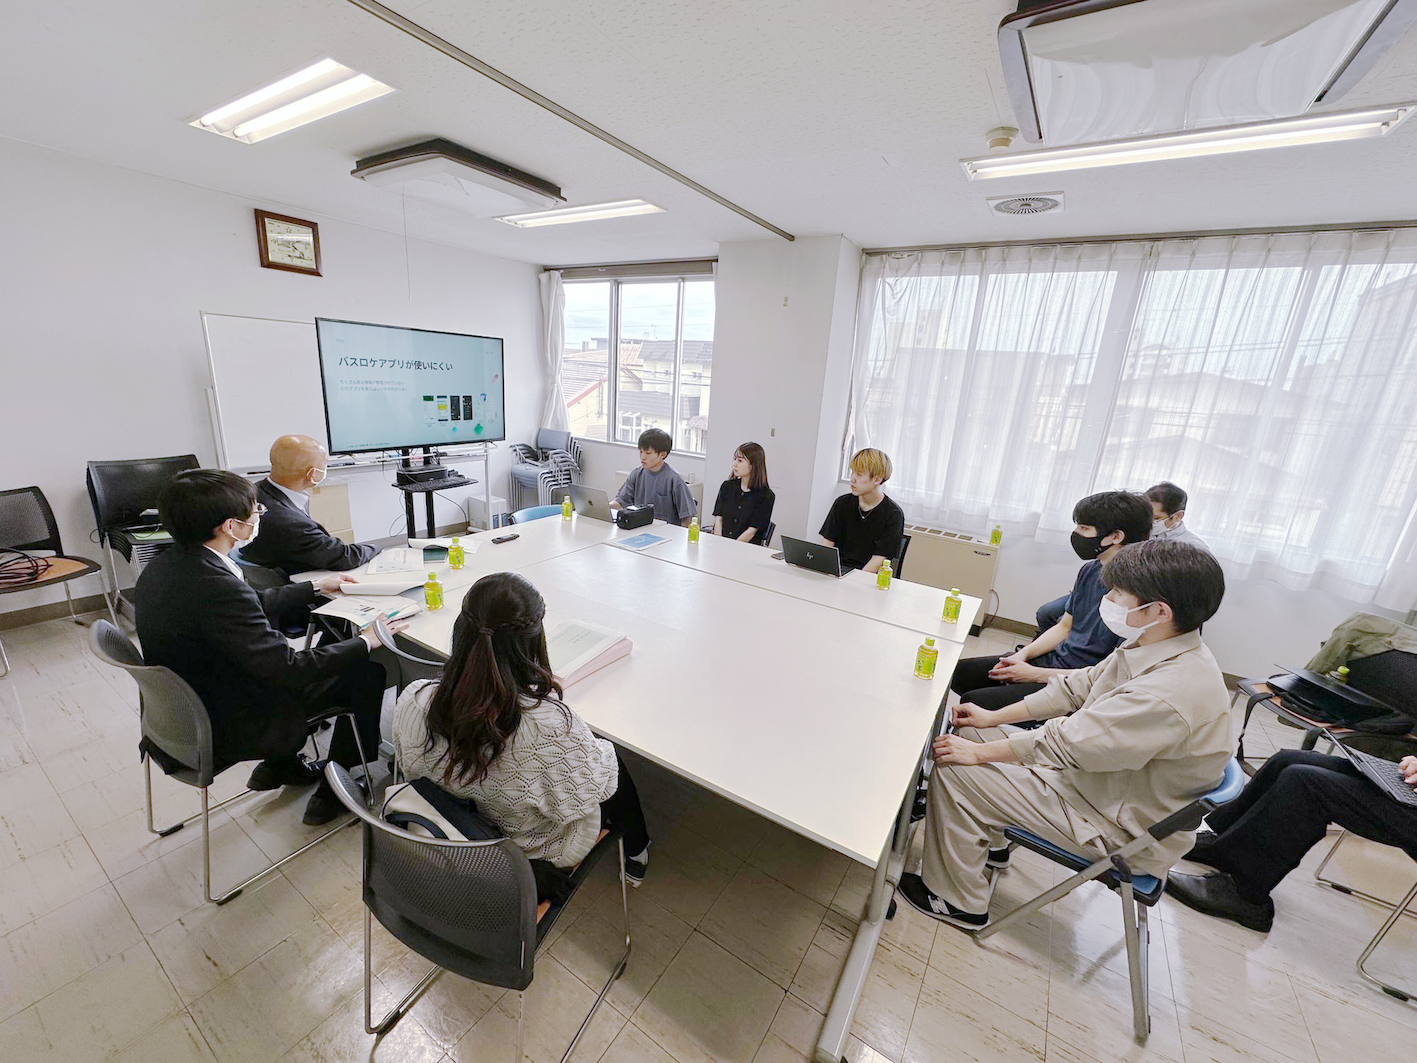
\includegraphics[width=9cm]{images/hakodate_bus.png}
    \caption{函館バス株式会社訪問時の様子}
    \label{fig:hakodate_bus}
\end{figure}
\bunseki{大津武琉}

\section{中間発表}
\subsection{中間発表資料の作成}
7月7日 (金) に行われる中間発表会に向けてスライド,メインポスター (図\ref{fig:interim_poster}) ,サブポスター (図\ref{fig:interim_poster_bulo}) を作成した.これらの資料に関して教員に繰り返しレビューをしていただき,より伝わりやすいものへと改良を重ねた.

\begin{figure}[H]
    \centering
    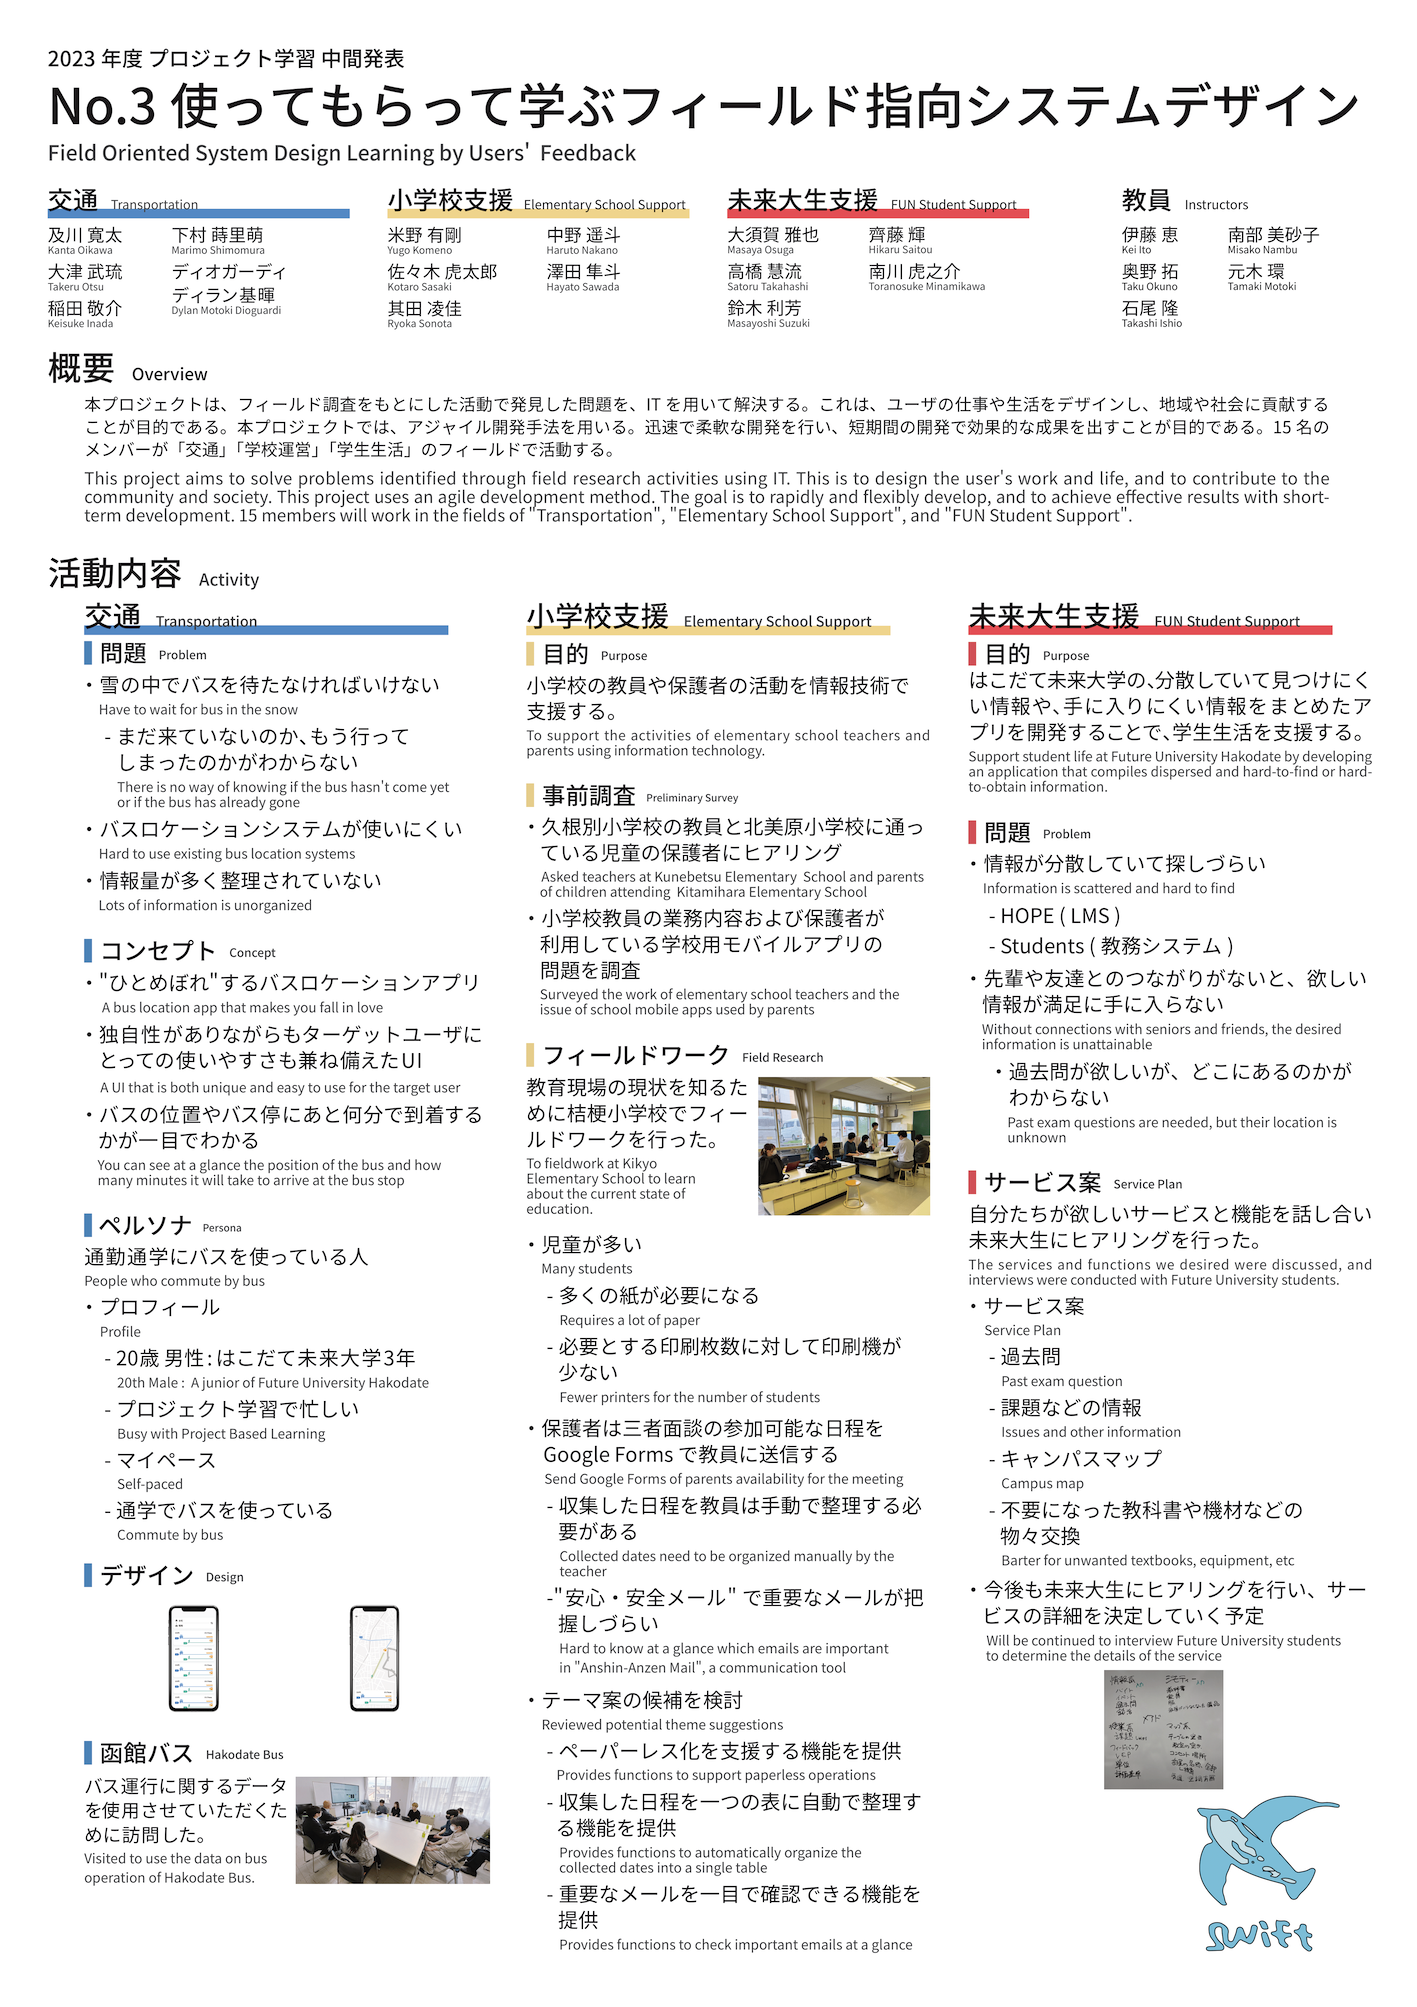
\includegraphics[width=14cm]{images/interim_poster.png}
    \caption{中間発表会メインポスター}
    \label{fig:interim_poster}
\end{figure}

\begin{figure}[H]
    \centering
    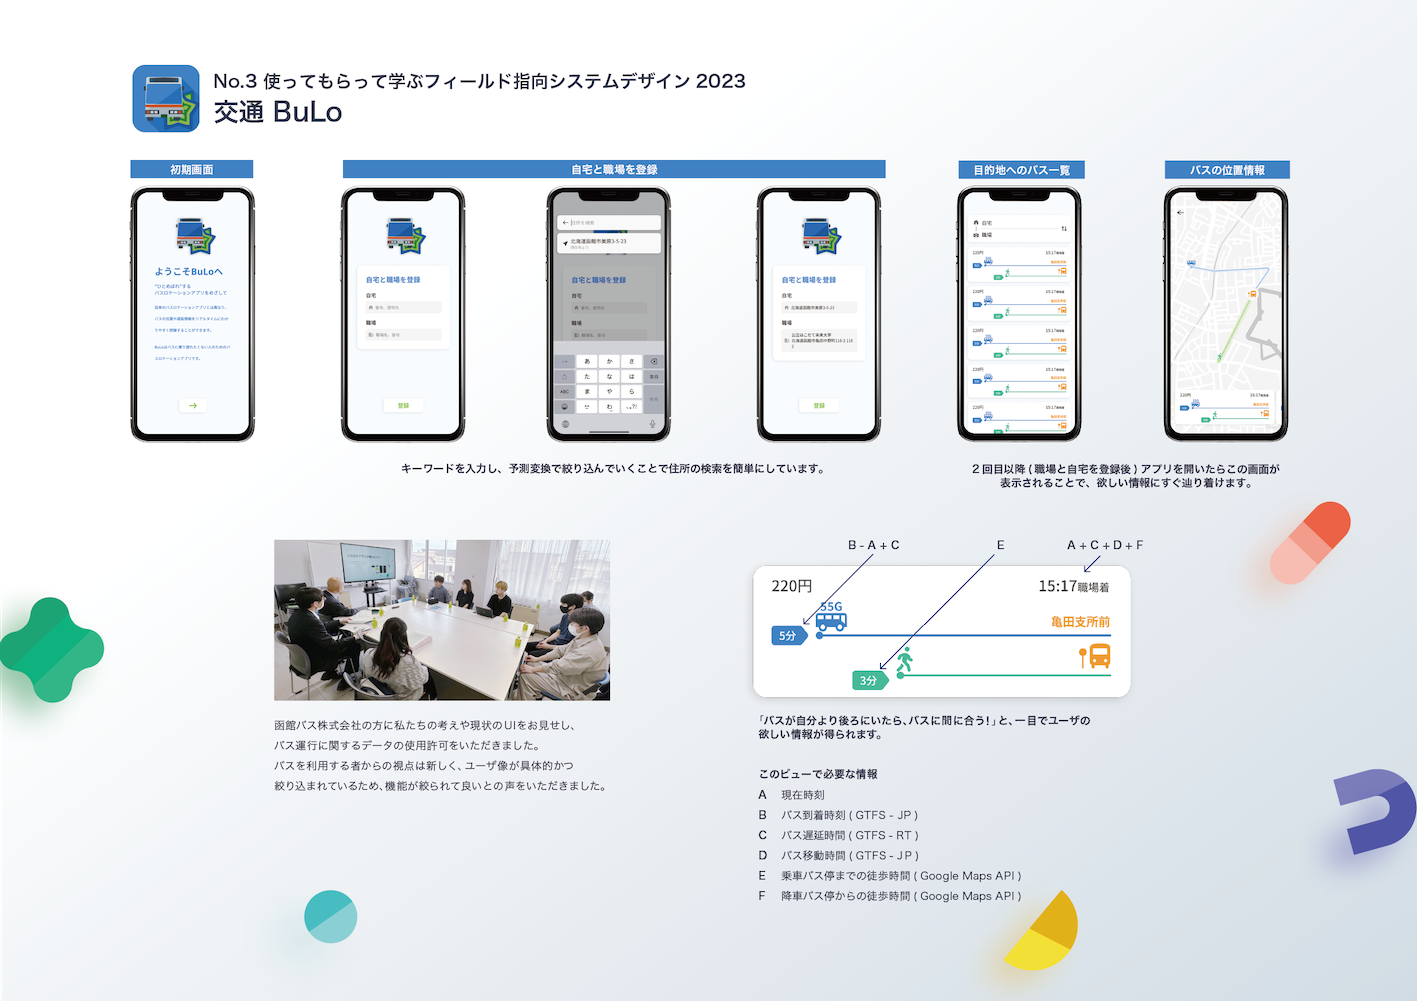
\includegraphics[width=14cm]{images/interim_poster_bulo.png}
    \caption{中間発表会サブポスター}
    \label{fig:interim_poster_bulo}
\end{figure}

\subsection{中間発表会}
7月7日 (金) に発表会は行われた.そこで様々な質問や意見をいただいた.「首都圏と函館で同じ状況を想定していいのか?」「独自性を掲げているがUIについての独自性のみで機能についての独自性がみられない」という指摘をいただいた.これらの意見は,ターゲットユーザを絞り,合わせて実装する機能を絞った結果であると考えているため,次期バージョンにて,いただいた指摘をもとに改善を行う.

\begin{figure}[H]
    \centering
    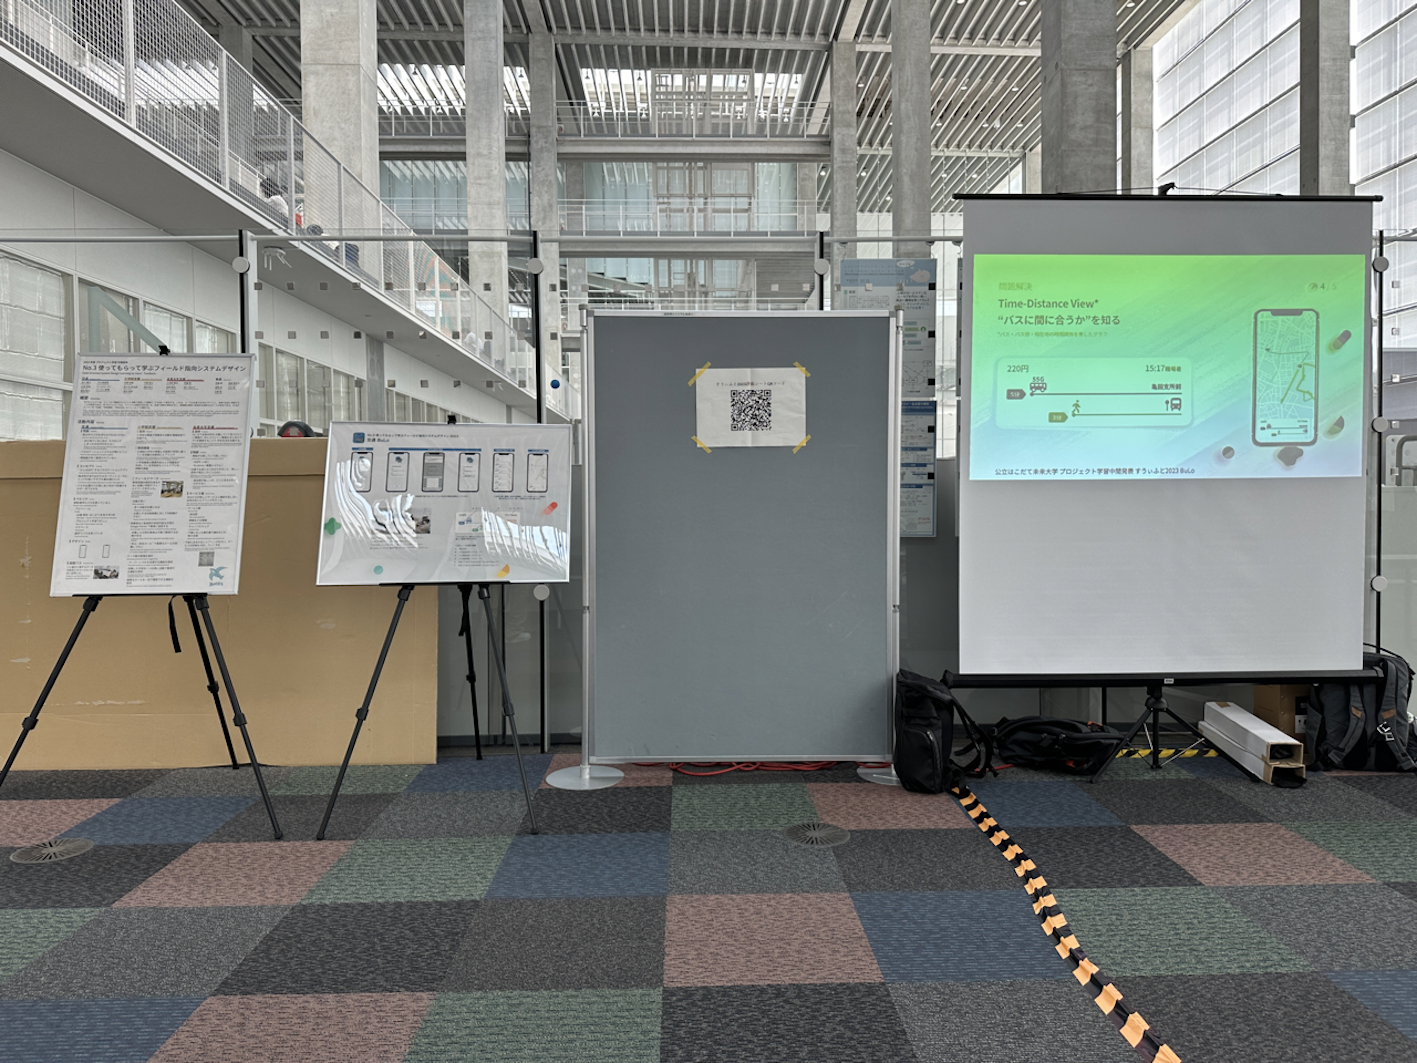
\includegraphics[width=12cm]{images/mid_presentation.png}
    \caption{中間発表会の様子}
    \label{fig:mid_presentation}
\end{figure}
\bunseki{下村蒔里萌}

\section{開発}
\subsection{アジャイル開発}
西村,永瀬,吉羽 (2020)によると,ソフトウェア開発において,目的を達成し,成果を最大化するための,以下のような進め方をアジャイル開発と呼ぶ \cite{scrum}.
\begin{quote}
    \begin{itemize}
        \item 関係者は目的の達成のためにお互いに協力し合いながら進める
        \item 一度にまとめてではなく少しずつ作り,早い段階から実際に動作するものを届け続けて評価を繰り返す
        \item 利用者の反応や関係者からのフィードバックを継続的に得ながら,作っているもの自体や計画を調整する
    \end{itemize}
\end{quote}

本サービスは,必要最小限の機能を実装した後,ユーザに使ってもらい,フィードバックを得る,というプロセスを繰り返しながら開発を行いたいという考えがあった.この考え,アジャイル開発を実現するために,我々は,アジャイル開発の手法の1つであるスクラムを用いて開発を行った.西村ら (2020) は,以下のようなスクラムの特徴を挙げている \cite{scrum}.

\begin{quote}
    \begin{itemize}
        \item 要求を価値やリスクや必要性を基準にして並べ替えて,その順にプロダクトを作ることで成果を最大化します
        \item スクラムでは固定の短い時間に区切って作業を進めます.固定の時間のことをタイムボックスと呼びます
        \item 現在の状況や問題点を明らかにします.これを透明性と呼びます
        \item 定期的に進捗状況やつくっているプロダクトで期待されている成果を得られるのか,仕事の進め方に問題がないかどうかを確認します.これを検査と呼びます
        \item やり方に問題があったり,もっとうまくできるよう方があったりすれば,やり方そのものを変えます.これを適応と呼びます
    \end{itemize}
\end{quote}

このようなスクラムは,5つのイベント,3つのロール,3つの作成物から構成されているとしている \cite{scrum}.

まず,プロダクトバックログ (作成物1) を作成する.プロダクトバックログとは,実現したい機能や,要求をリストアップし,実現したい順に並び替えたものである.常にメンテナンスして最新の状態を保つことが期待されている.

このプロダクトバックログを管理する責任を持つのは,プロダクトオーナー (ロール1; 以下,PO) である.POは,プロダクトの責任者であり,以下のような役割がある.
\begin{quote}
    \begin{itemize}
        \item プロダクトのビジョンを明らかにし,周りと共有する
        \item おおよそのリソース計画を定める
        \item 予算を管理する
        \item 顧客,プロダクトの利用者や組織の関連部署などの関係者と,プロダクトバックログの項目の内容を確認したり,作る順番や実現時期を相談したりする
        \item 既存のプロダクトバックログの項目の内容を最新の状態に更新する
        \item プロダクトバックログの項目の内容を関係者が理解できるように説明する
        \item プロダクトバックログ項目が完成しているかどうかを確認する
    \end{itemize}
\end{quote}

実際に作業を進めるのが,開発チーム (ロール2) である.開発チームは,短く区切られたスプリント (イベント1) ごとに開発を進める.スプリントプランニング (イベント2) で,プロダクトオーナーとともに,要求や実現可能性について議論する.

その後,スプリントバックログ (作成物2) を作成する.スプリントバックログとは,スプリントで実現する機能や,要求をリストアップし,実現したい順に並び替えたものである.スプリントバックログは,スプリントプランニングの終わりに作成される.

開発チームは,そのスプリントで,インクリメント (作成物3) を作成する.インクリメントとは,スプリントで実現した機能のことである.開発チームは,スプリントゴール達成に向けて進んでいるかどうかを,デイリースクラム (イベント3) で検査する.スプリントゴール達成に向けて昨日行ったこと,今日行うこと,障害となるものについて共有する.

スプリントの終わりに,スプリントレビュー (イベント4) とスプリントレトロスペクティブ (イベント5) を行う.スプリントレビューでは,スプリントで実現した機能をスクラムチーム外の関係者であるステークホルダに紹介し,フィードバックを得る.スプリントレトロスペクティブでは,開発チームのメンバが,スプリントでの作業の進め方や,やり方に問題がないかどうかを確認する.

これらのプロセスを円滑にまわして,プロダクトをうまく作れるように,POや開発チームを支えるのが,スクラムマスター (ロール3) である.

これらの基本原則を守りながら,開発を進めることで,アジャイル開発を実現した.

より効果的なアジャイル開発を行うために,デザインシステムの構築,スキーマ駆動開発を行なった.

\subsubsection{デザインシステム}
本サービスは,簡潔で見やすく情報量の絞られたデザインを目指している.そのために,サービス内で一貫したデザインを目指している.
また,アジャイル開発を行う上で,手戻りの少ない一貫性のあるUI改善を行うため,さらにはエンジニアとデザイナーの共通認識を図るために,
デザインシステムを導入した.
\bunseki{下村蒔里萌}

\subsubsection{スキーマ駆動開発}
APIのスキーマを元に,クライアントサイド,サーバサイド,デザイナーの3者間で,共通の認識を持ち,開発を進めた.デザイン変更に伴う,機能変更の際も,スキーマを元に話を進めるため,スムーズに柔軟な開発を進めることができた.
\bunseki{及川寛太}

\subsection{使用した技術}
\subsubsection{Flutter}
当初は,iOSアプリをSwiftで,AndroidアプリをKotlinで開発する予定であったが,開発期間が短いことや人数が少ないことから,1つのコードベースで2つのプラットフォームをサポートできる,Flutterを採用した.

\subsubsection{GraphQL}
本サービスでは,当初,GraphQLサーバを介して,バックエンドのマイクロサービスと通信していた.
GraphQLのデメリットや,マイクロサービス間では,gRPCによる通信が行われていたことから,gRPCを用いて通信するように変更した.

\subsubsection{gRPC}
本サービスでは,マイクロサービス間通信,および,バックエンドのマイクロサービスとクライアント間通信にgRPCを用いている.

\subsubsection{PostgreSQL}
本サービスでは,GTFS-JPの静的データを保存し,各サービスからアクセスするために使用した.

\subsubsection{Google Cloud Platform}
本サービスの,データベースサーバはCloudSQL\footnote{https://cloud.google.com/sql/},バックエンドのマイクロサービスはCloud Run\footnote{https://cloud.google.com/run/}上で稼働している.
サーバレスサービスにより,サーバの管理にリソースを割くことなく,開発に集中することができる.
\bunseki{及川寛太}

\subsection{使用したツール}
\subsubsection{Discord}
本グループでは,コミュニケーションツールとしてDiscord\footnote{https://discord.com/}を使用した.
テキストチャットと音声チャットを使用し,グループ内での進捗共有や,デイリースクラムを行った.
開発中のコードに対しての質問や相談は,後述するGitHubやFigmaのコメント機能を使用した.
簡単な質問や相談,雑談についてはDiscordを使用した.
\bunseki{下村蒔里萌}

\subsubsection{Figma}
本サービスのプロトタイプはFigma\footnote{https://www.figma.com/}で作成した.
これは,Figmaのオートレイアウトやコンポーネント機能を使用することで,プロトタイプの作成とエンジニアとの連携を効率化するためである.
また,Figmaの共有機能を使用し,開発に入る前にステークホルダーにプロトタイプを使用してもらい,フィードバックをもらった.

また,本サービスのデザインシステムの作成にもFigmaを使用した.
Figmaのローカルバリアブルやローカルスタイル機能を使用することで,デザインシステムの作成とエンジニアとの連携を効率化した.
Figma内でデザインシステムとプロトタイプを完結させることで,プロトタイプの保守運用を効率化した.
\bunseki{下村蒔里萌}

\subsubsection{GitHub Projects}
本サービスのプロダクトバックログ,スプリントバックログ,詳細なタスク管理については,GitHub Projects\footnote{https://docs.github.com/issues/planning-and-tracking-with-projects/learning-about-projects/about-projects}を使用した.開発リポジトリのIssueやPull Requestと連携することで,見通しを確保し,開発の進捗管理を効率化した.
\bunseki{及川寛太}

\subsubsection{Notion}
Notion\footnote{https://www.notion.so/}を使用して,ドキュメントの管理を行った.ミーティングの際の議事録や,知識の集約,日報の記録などを行なった.見通しを良くするために,ページのナビゲーションやレイアウトを工夫した.
\bunseki{及川寛太}

\section{UCDワークショップ}
9月17日 (日) ,9月18日 (月) に希望するメンバでUCDワークショップに参加した.
UCDワークショップとは,高度IT人材を育成する産学協働の実践教育ネットワーク ``enPiT''\footnote{https://www.enpit.jp/}の取り組みの1つである.
このワークショップでは,大阪芸術大学のアートサイエンス学科で教鞭をとる准教授である大塚あゆみ氏を講師としてお招きし,人間中心のデザイン,ユーザ・センタード・デザイン (それぞれの頭文字を取ってUCD) の考え方とその設計方法を,短期集中の講義と演習を通して学んだ.
演習では,20年後の未来で使いたい製品・サービスを考え,シナリオ形式で発表した.
ここではグループメンバとコミュニケーションを円滑に図るために,ビジュアルシンキングを用いてアイディアを共有した.
城川 (2018) によると,ビジュアルシンキングとは,あたりまえなことに疑問をもって観察し,それを視覚的に記録することである\cite{visual}.
また,ヒューマン・センタード・デザイン (HCD) を意識して避けるなど,随時アイデアを評価しながら洗練されたものにしていくまでの手順を実践した.
\bunseki{稲田敬介}

\section{アカデミックリンク}
11月3日 (金) にはこだて高等教育機関合同研究発表会,通称HAKODATEアカデミックリンクに参加した.HAKODATEアカデミックリンクは,函館市内にある8つの大学,短大,高専で日々行われる研究を市民・地元企業の方々にわかりやすく披露する場として提供されたものである.
今年度のHAKODATEアカデミックリンク2023は函館アリーナで4年ぶりに対面で開催され,キャンパス・コンソーシアム函館に加盟する8校の学生をはじめ,函館市内の高校生や他地域の大学生などが参加した.
ここでは,情報系である方やそうでない方など,様々な分野に進んだ方々が参加していたのに加え,バスを普段の生活で使っている方,そうでない方など,様々な属性を持った方々がいらっしゃったため,多様な評価をいただくことができた.
\bunseki{稲田敬介}

\section{成果発表会}
\subsection{成果発表会資料作成}
12月8日 (金) の成果発表会に使用するプロジェクト全体用のメインポスター,グループ発表用のグループポスター,発表スライドを作成した.これらの資料は教員に随時レビューを求め,わかりやすい資料になるよう改良を重ねた.

\begin{figure}[H]
    \centering
    \includegraphics[width=14cm]{images/final_main_poster.png}
    \caption{成果発表会メインポスター}
    \label{fig:final_main_poster}
\end{figure}

\begin{figure}[H]
    \centering
    \includegraphics[width=14cm]{images/poster.png}
    \caption{成果発表会サブポスター}
    \label{fig:poster}
\end{figure}

\bunseki{稲田敬介}

\subsection{概要}
12月8日 (金) に成果発表会が行われ,そこでは未来大内外問わず,様々な方々からな意見や質問をいただくことができた.
説明資料としてブースに配置していたポスター,デモ機,また,発表とそれに用いたスライド等を通して,「TDViewにリスト表示されている分数を表すゲージの長さは,相対的に決めるのでは分かりづらいのではないか?」といったUIに関する意見や,「データの管理方法や精度はどのようになっているのか」など,データの取扱に関する質問をいただくことができた.
またその一方で,「このアプリがリリースされたら使いたい」といったニーズが存在することを確認できた.
\bunseki{稲田敬介}

\section{enPiT BizSysD 北海道・東北合同発表会}
12月9日 (土) にWebとZoom上にて行われた,enPiT BizSysD 北海道・東北合同発表会に参加した.この発表会はいくつかの他大学と合同で行われ,全8チームのエントリーとなった.
発表資料としては,前日に行われた成果発表会にて使用した資料をそのまま用いた.
発表を通して教員・学生等様々な方々から評価をしていただくことができ,アイデア部門の最優秀賞,全体を通しての最優秀賞を受賞した.
また,他大学の利用する技術,アイデア等を拝見できる貴重な機会として,充実した発表会となった.
\bunseki{稲田敬介}

\chapter{今後の予定}
今後の予定は,1つ目に,複数事業者に対応させることを目指す.現状のバージョンでは函館バスのみしか対応していない.これを拡張し,函館市電やJR,また函館市以外のバス事業者にも対応させる.2つ目に乗り換えに対応させることを目指す.バスを利用する上で目的地まで行くのに乗り換えが起こることは多くある.また,すでに「乗り換えに対応して欲しい」という指摘が多く寄せられているので乗り換えに対応させることをを目指す.3つ目にパフォーマンスの向上を図る.現状のバージョンでは,住所を検索する際や,路線を検索する際,結果が出るまでに時間がかかってしまっている.本サービスは「ひとめぼれ」をコンセプトとしているため,このレスポンスの遅さを改善することを目指す.4つ目に,Route Viewでのルートの表示を目指す.ユーザのルートの表示の目処は立っている.しかし,函館バスが提供しているデータの中に,ルートの情報がないため,バスのルートの表示の目処が立っていない.そこでどのようにしてルートを表示するかを考え,実装を行う.最後に,調査に基づいてUI/UXの改善を行う.すでに中間発表会や成果発表会でUI/UXの改善点を指摘された.それらの指摘に加えて,一般リリースをしたあとの,ユーザのフィードバックをもとに改善を行い,より使いやすいアプリにしていく.
\bunseki{大津武琉}
\chapter{学び}

\section{個人の学び}
\subsection{稲田敬介}
\bunseki{稲田敬介}

\subsection{及川寛太}
\bunseki{及川寛太}

\subsection{大津武琉}
\bunseki{大津武琉}

\subsection{下村蒔里萌}
\bunseki{下村蒔里萌}


\chapter{まとめ}
本グループでは,バス利用者がストレスを抱えずにバスをできるようなアプリ「BuLo(ブーロ)」の開発を行った.最初にブレインストーミングを行い,メンバそれぞれがやりたいことについて話し合った.その中で,公共交通機関が利用しづらい問題を解決したいという意見が出た.その意見に対してメンバの多くが共感し,本グループの開発するプロダクトを決定した.次に,プロトタイプの作成を行い,プロジェクトメンバによるユーザテストを行なった.その結果,ターゲットユーザが定まっておらず,本サービスは何のため,誰のためのアプリなのかがわからないことに気がついた.そこで,本サービスについてもう一度考え直すことでターゲットユーザを確立させ,それをもとにプロトタイプを改善した.本サービスで函館バス株式会社のデータを利用するために,本サービスの紹介とデータ使用を願い出に,函館バス株式会社を訪問した.そこで,「新しい観点からの機能で良い」という感想をいただいた.その後,プロトタイプをもとにクライアントサイド,サーバサイドそれぞれ開発を進めていき,中間発表会では,その時点での開発状況を発表し,プロトタイプを用いてデモを行なった.そこで,機能やUIについての指摘をいただき,それをもとに本サービスの改善を行なった.再びクライアントサイド,サーバサイドそれぞれで開発を進めた後,はこだて高等教育機関合同研究発表会で本サービスについての発表を行なった.そこでは,情報系を専門としていない,市民や高校生などの一般の方々からも意見や質問をいただくことできた.その後,本サービスの開発を進め,成果発表会にて,本サービスの最終発表を行なった.そこでは,未来大学関係者や函館市民,企業の方々と多くの方に本サービスに興味を持っていただくことができた.また,様々な観点からの意見や質問をいただくことができ,本サービスの改善に繋げることができた.現状では,本サービスの一般リリースを行うことがきていないが,様々な発表を通じて本サービスのニーズがあることを確認できているため,今後も開発を進めて一般リリースを目指していきたい.
\bunseki{大津武琉}


\begin{appendix}
\chapter{使用した技術・ツール・知識}

\section{フレームワーク}
\subsection{Flutter}
モバイルアプリのフレームワークとしてFlutter\footnote{https://flutter.dev/}を用いた.Android,iOSの両者にサービスを展開する上でKotlin,Swiftそれぞれでネイティブアプリを作成する事も検討したが,グループの規模とメンバーの技術力を考慮して,クロスプラットフォーム開発が可能であるFlutterを用いることに決定した.

\section{ツール}
\subsection{Discord}
本グループの主な連絡手段としてDiscord\footnote{https://discord.com/}を使用した.プロジェクトの連絡はもちろん,日常生活で起こったことなどをDiscordで共有することによりチームワークの向上を実現することができた.

\subsection{Notion}
本グループでは情報を管理するツールとしてNotion\footnote{https://www.notion.so/}を使用した.議事録,日報,週報,プロダクトバックログをそれぞれページにまとめることにより,情報を見やすくすることができた.今後も情報の管理ツールとして使用をしていく.

\subsection{GitHub}
GitHub\footnote{https://github.com/}とはソースコードのバージョン管理システムである.このツールを用いることでチームでのアプリ開発を効率的に行うことができる.本グループではフロントエンド,バックエンドでそれぞれリポジトリを作成し,アプリの開発を進めている.今後はより一層アプリの開発を進めることとなるため,GitHubを利用していく.
\pagebreak
\subsection{Figma}
Figma\footnote{https://www.figma.com/}とは,ホームページやアプリケーションなどのワイヤーフレームを作成できるツールである.中間発表スライドの作成,プロトタイプの作成,函館バス訪問の際に使用したスライドの作成に使用した.コンポーネントやレスポンシブを意識し,ワイヤーフレームを作成することで,今後の開発がスムーズになるようにした.

\subsection{Slack}
本プロジェクトの主な連絡手段としてSlack\footnote{https://slack.com/}を使用した.本グループでは主な連絡手段としてDiscordを利用していたが,プロジェクトではSlackを利用するとなったため使用した.細かくチャンネルを分けることで情報がどこにあるかをわかりやすくすることができた.また,メンションという機能を利用することにより教員,プロジェクトメンバー,TAとそれぞれに通知が行くようにすることで効率の良い意思疎通を行うことができた.

\subsection{Miro}
Miro\footnote{https://miro.com/}はオンラインでホワイトボードを利用できるツールである.ブレインストーミングなど,メンバーで一斉に意見を書くときに使用した.Miroを使用することにより,メンバーそれぞれの意見,考えを効率よく共有することができた.現在は同じような機能を持ったFigJamを利用している.

\subsection{FigJam}
FigJam\footnote{https://www.figma.com/}はオンラインでホワイトボードを利用できるツールである.Miroと同じようなツールだが本グループではFigmaを利用しており同じサービス元であるためFigJamへと移行した.

\subsection{Google Drive}
Google Drive\footnote{https://drive.google.com}とはGoogleが提供するオンラインストレージサービスである.これを用いることにより手軽にファイルの共有を行うことができる.また昨年度のファイル履歴を見返すこともでき,資料作り,プロジェクトの進め方の参考とした.
\pagebreak
\section{マネジメント}
\subsection{リスクマネジメント}
プロジェクトを行ううえでリスクは必ず存在する.リスクマネジメント\cite{risk}はそのリスクに対してどのように対策するのかを考える.まず初めにプロジェクトメンバーを3グループに分け,それぞれのチームでメンバーが持ち寄った起こりそうなリスクをまとめた.その後それぞれのリスクに対して,そのリスクが被る被害,発生確率,影響度,脅威,対策を考えた.脅威については発生確率,影響度を掛け合わせたものであり,脅威の値が大きいほど対策するべき優先度が高いものとなる.

\chapter{活用した講義}
\section{アジャイルワークショップ}
アジャイルコーチの永瀬氏に,本プロジェクトで用いるチーム開発の手法であるアジャイル開発について講義をしていただいた.まず,本ワークショップの前に事前知識を得るため,アジャイル開発についてのビデオを視聴した.その知識をもとに永瀬氏からアジャイル開発とはなにか,アジャイル開発で用いられるスクラムとはなにかを学んだ.また,最後に講義を受けているメンバーを5人ずつのチームにし,スクラムについてのクイズ大会を行った.これにより,楽しみながらスクラムについて学ぶことができ,スクラムについての共通認識を持つことができた.

\section{フィールドワーク講座}
本プロジェクトの担当教員でもある,南部美砂子准教授,元木環准教授に講義をしていただき,フィールドワークに関する基本的な考え方,ありがちな間違いをご教授いただいた.収束的なフィールドワークでは,思い込みや認識の狭さなどを超えられないため,フィールドワークには問題を探しにいくのではないこと,また,人々の行為や相互行為には必ず理由や動機が存在し,それらを理解することをフィールドワークの目的とすることを学んだ.

\bunseki{稲田敬介}

\chapter{夏季休暇中の活動}

\bunseki{稲田敬介}
\end{appendix}

\begin{thebibliography}{3}
    \bibitem {scrum} 西村 直人, 永瀬 美穂, 吉羽 龍太郎. SCRUM BOOT CAMP THE BOOK スクラムチームではじめるアジャイル開発. 株式会社 翔泳社. 2020.
    \bibitem {scrummaster} Zuzana Sochova. SCRUM MASTER THE BOOK. 株式会社 翔泳社. 2020.
    \bibitem {risk} 株式会社インターリスク総研,リスクマネジメント入門. \url{https://www.ms-ins.com/pdf/business/rm/rmguide.pdf} (2023/07/12)
\end{thebibliography}
\end{document}
